\appendix 
\makeatletter
\addtocontents{toc}{\protect\renewcommand\protect\cftchappresnum{\@chapapp\ }}
\makeatother
\renewcommand{\thechapter}{\Alph{chapter}}

\chapter{Rescaled Range and Auto-Correlation Analysis for Measuring Bursts} \label{chap:appendix-valinor}


\section{Rescaled-range analysis for estimating H}
\label{app:rs}
For a weak stationary stochastic process $X = (X_t : t = 0, 1, 2, ..., N )$, the mean-adjusted series is defined as $Y$, $Y_t = X_t - m$ where $m$ is the empirical mean of the process $X$.
Let $Z$ denote the cumulative deviate of $Y$ where $Z_t = \sum_{t=1}^{N} Y_t$. We also define $m_t$ as the cumulative mean of the series $X$ through time $t$.

The rescaled range of $X$ is denoted by
\begin{equation}
    (R/S)_t = \frac{R_t}{S_t}, t \in \{0, 1, 2, ..., N\}
\end{equation}
where the Range series $R$ is defined as
\begin{equation}
\begin{split}
    R_t = Max(Z_1, Z_2, ..., Z_N) - Min(Z_1, Z_2, ..., Z_N), \\
    t \in \{0, 1, 2, ..., N\}
\end{split}
\end{equation}

and the standard deviation series $S$ is defined as
\begin{equation}
\begin{split}
    S_t = \sqrt{\frac{1}{t} \sum_{i = 1}^{t} (X_i - m_t)^2 },
    t \in \{0, 1, 2, ..., N\}
\end{split}
\end{equation}
According to \cite{hurst}, $R/S$ scales with the power law of $t$. Therefore, to estimate $H$, the slope of the least-squares linear regression of $R/S$ over $t$ in a log-log scale is used.
The resulting exponent is in the 0-1 range and a value between 0.5 to 1 indicates low to strong long-range dependence (self-similarity), respectively. 
In other words, an H estimate close to one indicates a strong desire to maintain the previous trend or more burstiness. As the H estimate nears 0.5, the time series becomes indistinguishable from random noise, and a value close to zero signifies the traffic's aim at reverting to its mean value.

\begin{figure}[th!]
	\centering
	\begin{subfigure}[t]{0.75\linewidth}
	\centering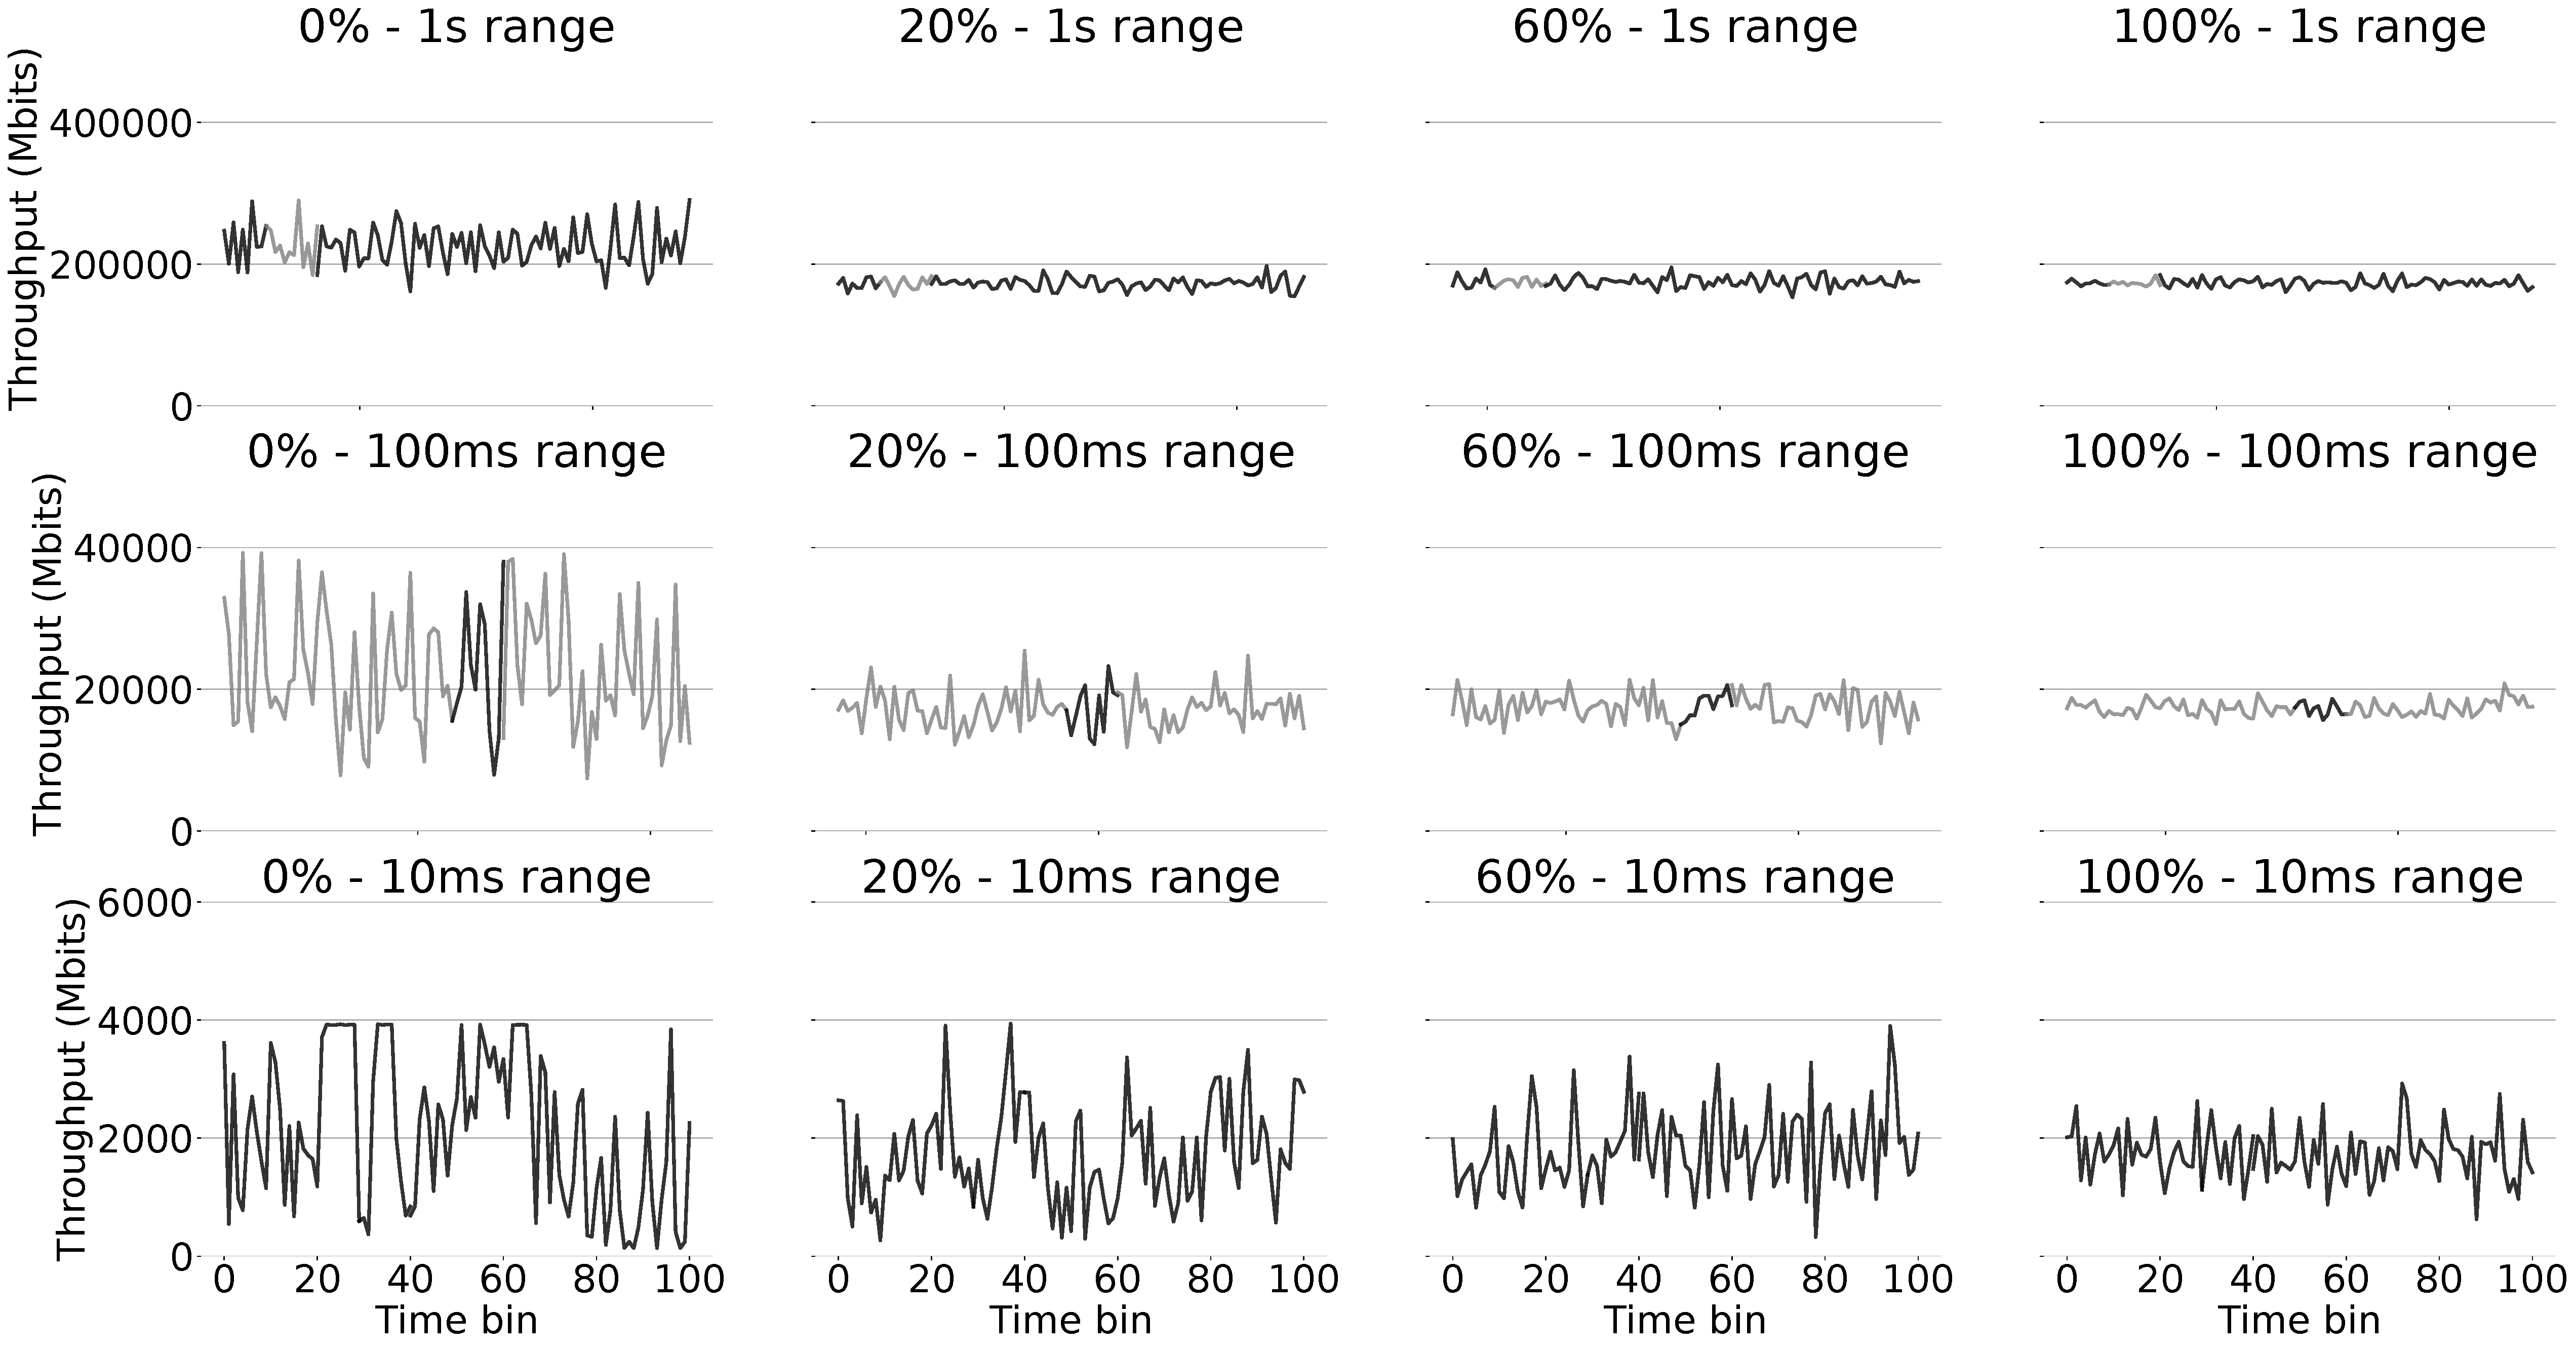
\includegraphics[width=1\linewidth]{figs/intra_cluster_byte_time_series.pdf}
    \caption{\small{\textbf{Intra-cluster time series}}}
    \label{fig:app-pacing-ts-cluster}
			% \vspace{-2mm}
    \end{subfigure}
    	\begin{subfigure}[t]{0.75\linewidth}
	\centering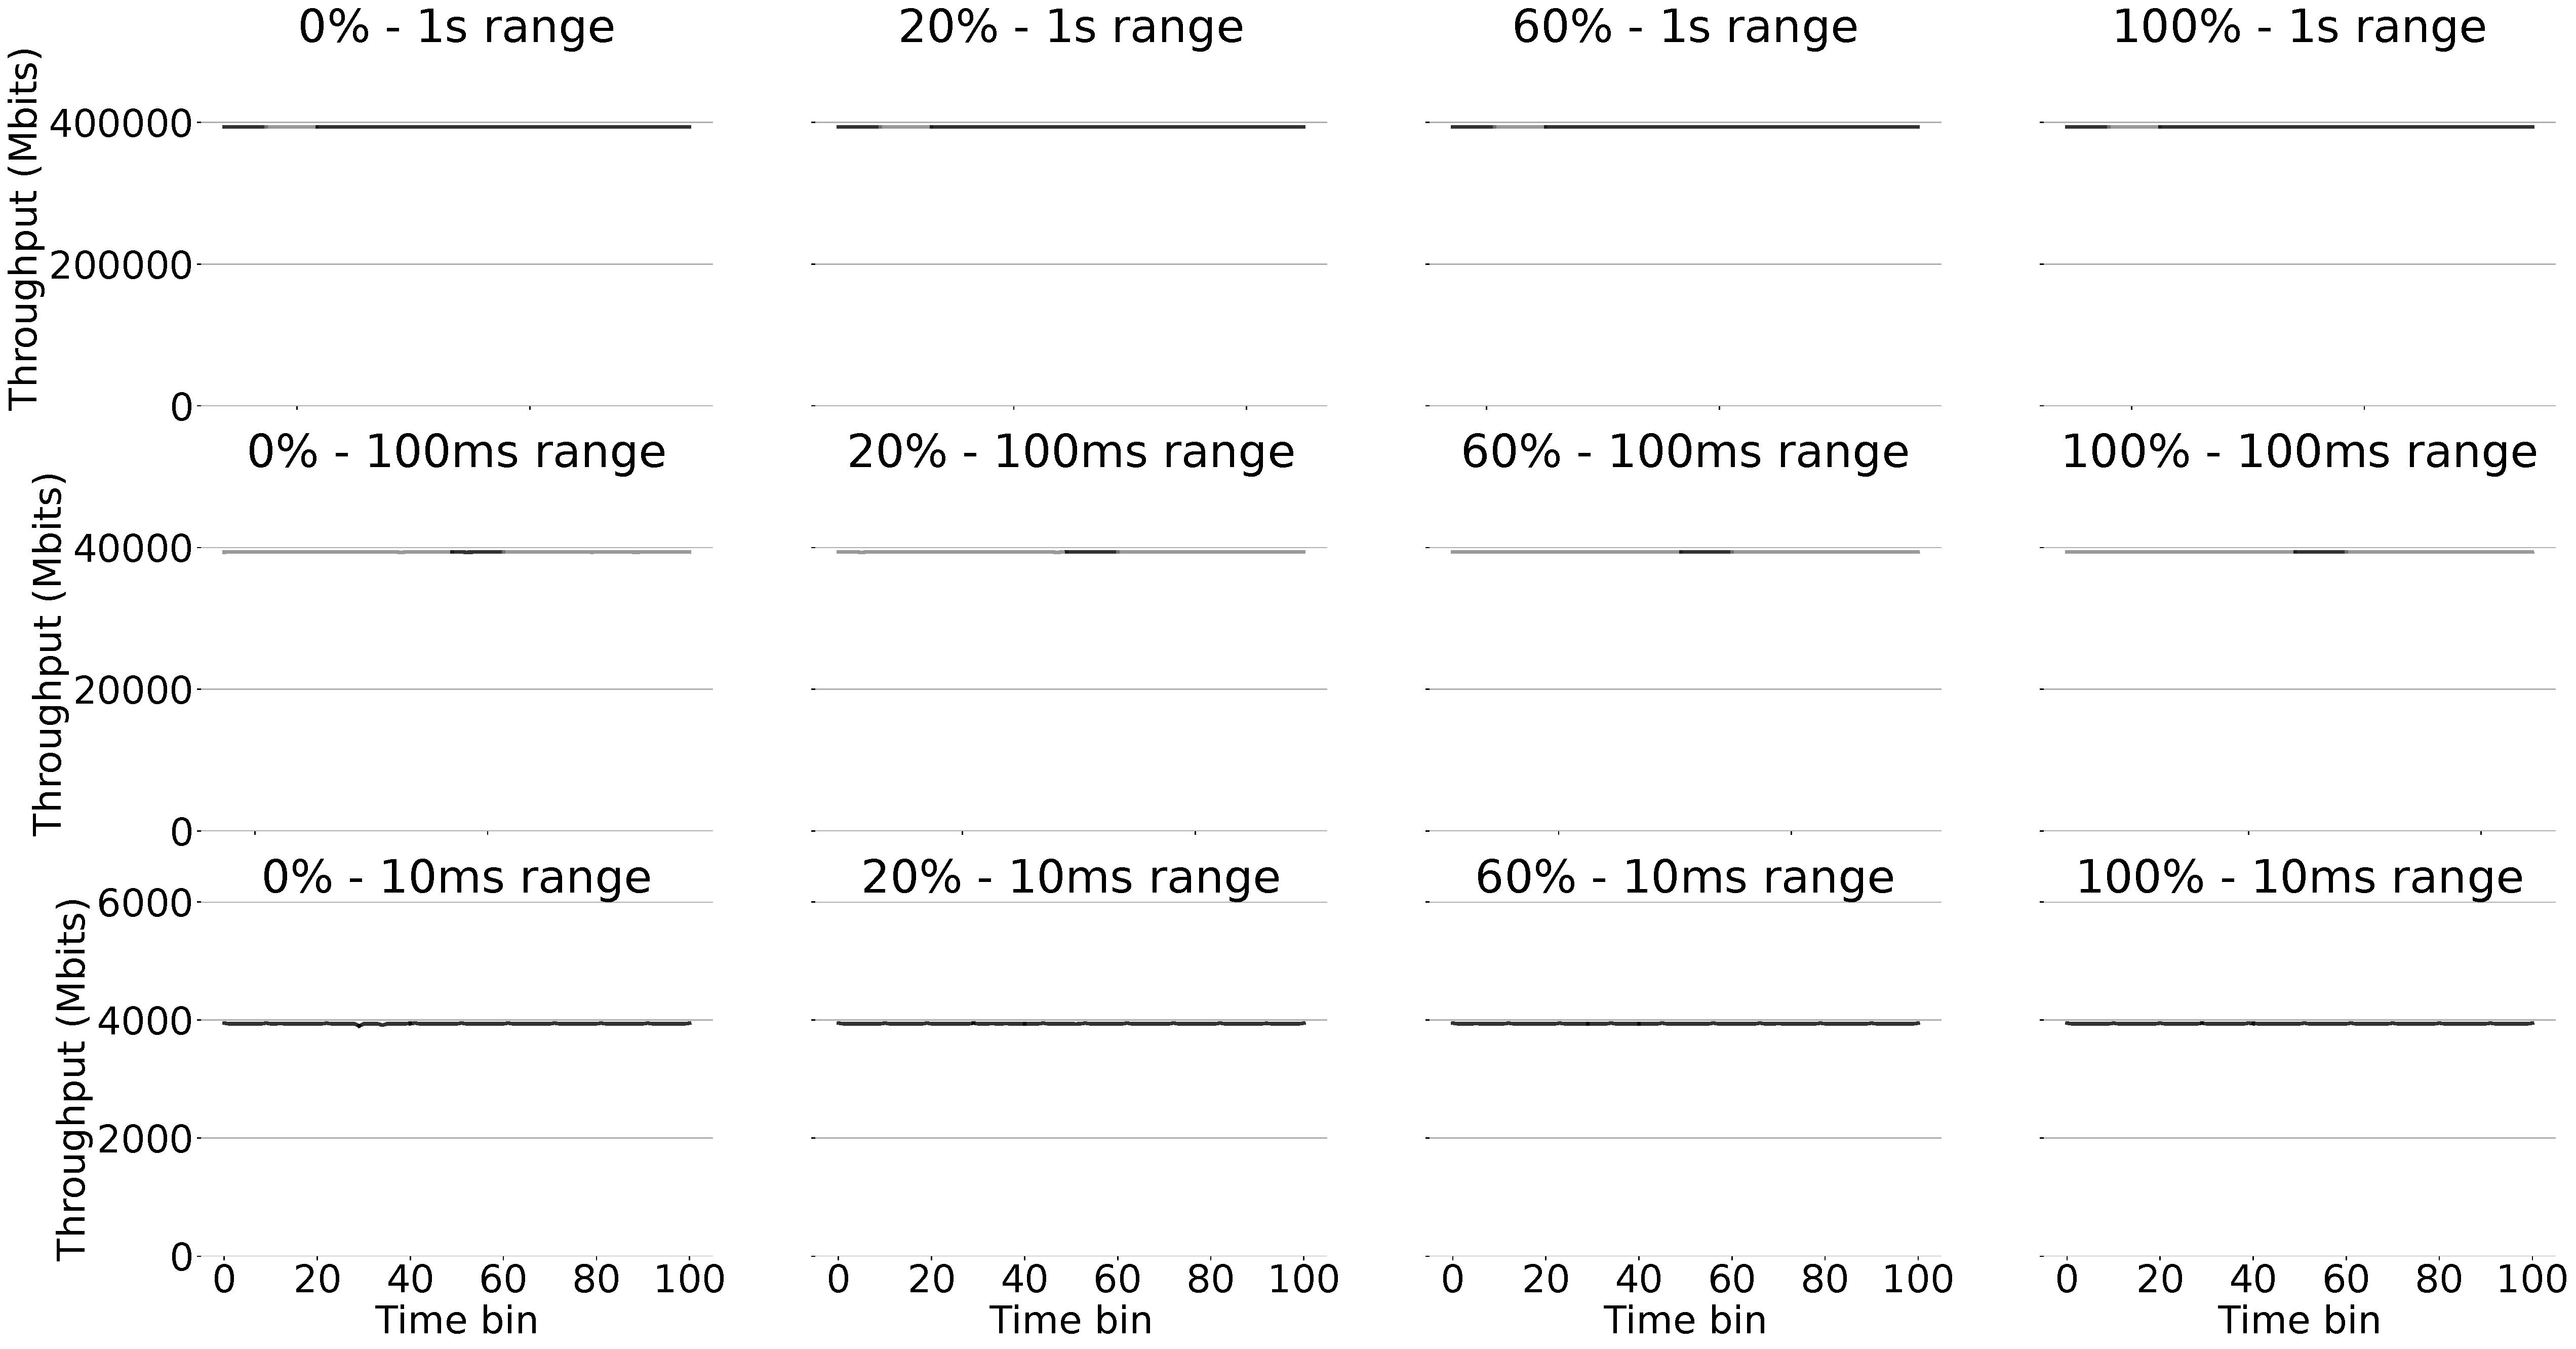
\includegraphics[width=1\linewidth]{figs/intra_rack_byte_time_series.pdf}
    \caption{\small{\textbf{Intra-rack time series}}}
    \label{fig:app-pacing-ts-rack}
			% \vspace{-2mm}
    \end{subfigure}
    \caption{\small{Time-series graphs for the software pacing experiments presenting the traffic behavior at three time ranges.}}
        \label{fig:app-pacing-ts}
         \vspace{-2mm}
\end{figure}

\begin{figure}[t]
	\centering
	\centering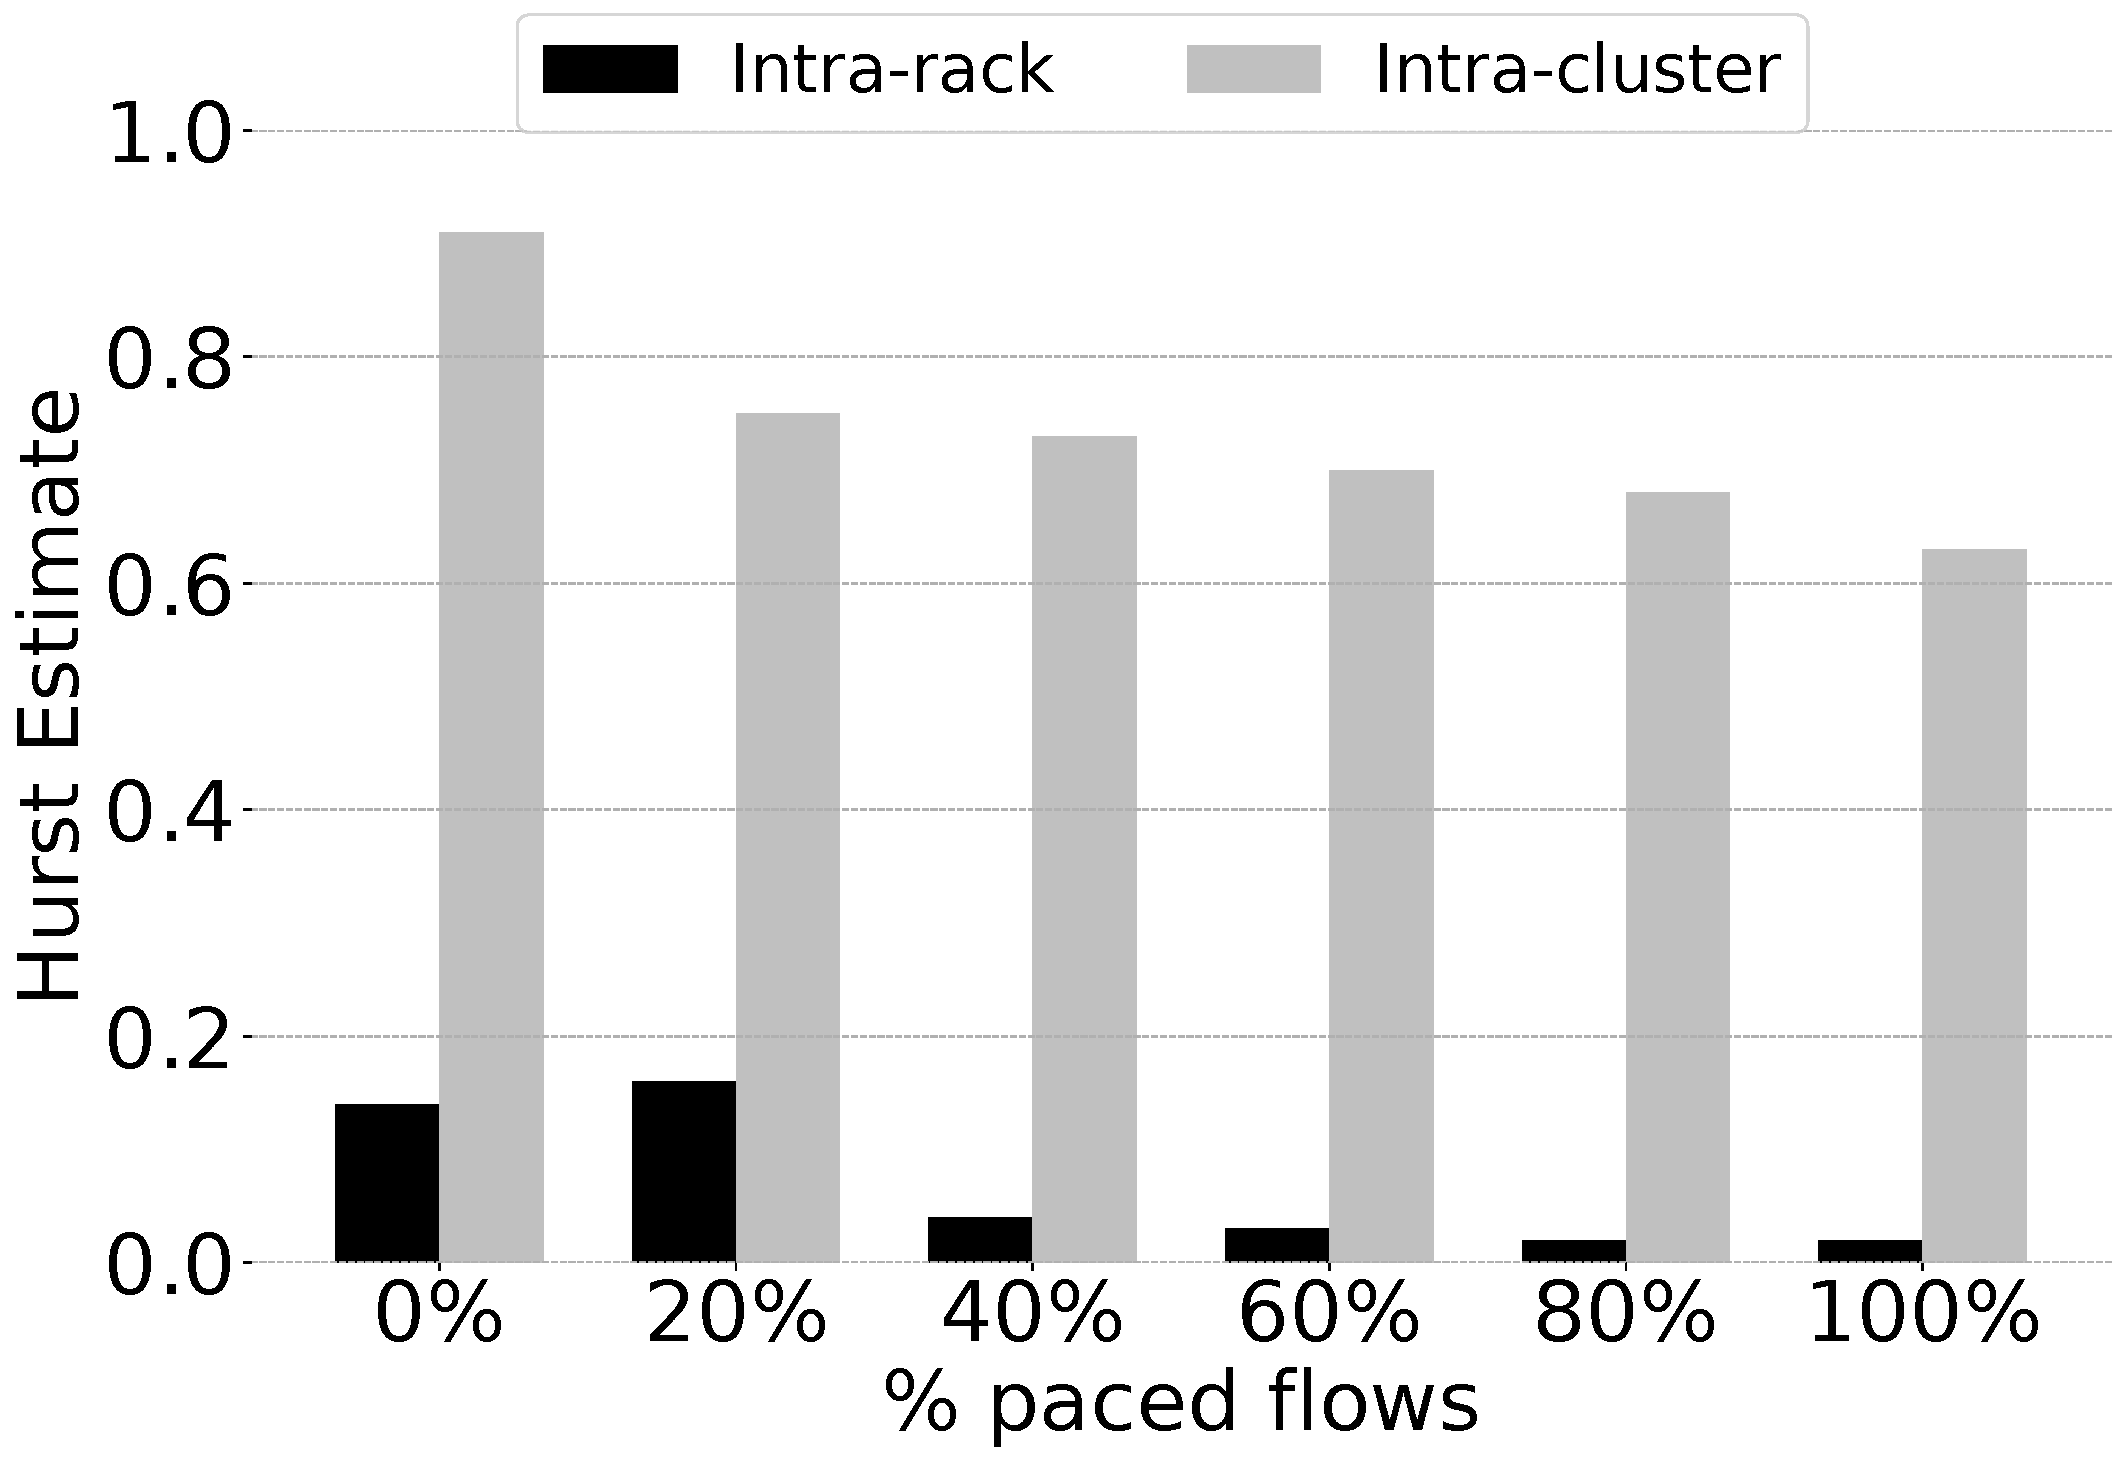
\includegraphics[width=0.65\linewidth]{figs/pacing_hurst_bar.pdf}
    \caption{\small{Hurst exponents for different degrees of software pacing.}}
        \label{fig:app-pacing-hurst}
         \vspace{-2mm}
\end{figure}

\section{Theoretical Analysis of Software Pacing Under Different Workloads}
\label{sec:app-pacing}
We presented the size of per-flow bursts for explicit software pacing in \S\ref{sec:pacing}. To further verify our findings using the notion of self-similarity, we first plot the time-series of packet arrivals in 1s, 100ms, and 10ms time scales in Figure \ref{fig:app-pacing-ts} for both the intra-cluster (Figure \ref{fig:app-pacing-ts-cluster}) and intra-rack (Figure \ref{fig:app-pacing-ts-rack}) workloads. One can notice the gradual decay of burstiness in all time scales as higher degrees of pacing are enforced to the intra-cluster workload. On the other hand, we can observe that the intra-rack traffic follows a non-bursty, steady trend in all time scales regardless of pacing.

Next, we calculate the Hurst exponents for the intra-rack and intra-cluster workloads. According to Figure \ref{fig:app-pacing-hurst}, self-similarity in the latter workload follows the degree of pacing (i.e., percentage of the paced flows) where 100\% pacing results in 31\% reduction in the Hurst estimate compared to the no-pacing case. For example, the Hurst estimates are 0.91, 0.73, and 0.63 for 0\%, 40\%, and 100\% pacing ratios, respectively. However, under the intra-rack workload pacing seems to have little to no effect as the egress traffic follows a mean-reverting behavior during 1-second time ranges (H < 0.20 for all the cases).



% \begin{figure}[th!]
% 	\centering
% 	\begin{subfigure}[t]{.80\linewidth}
% 	\centering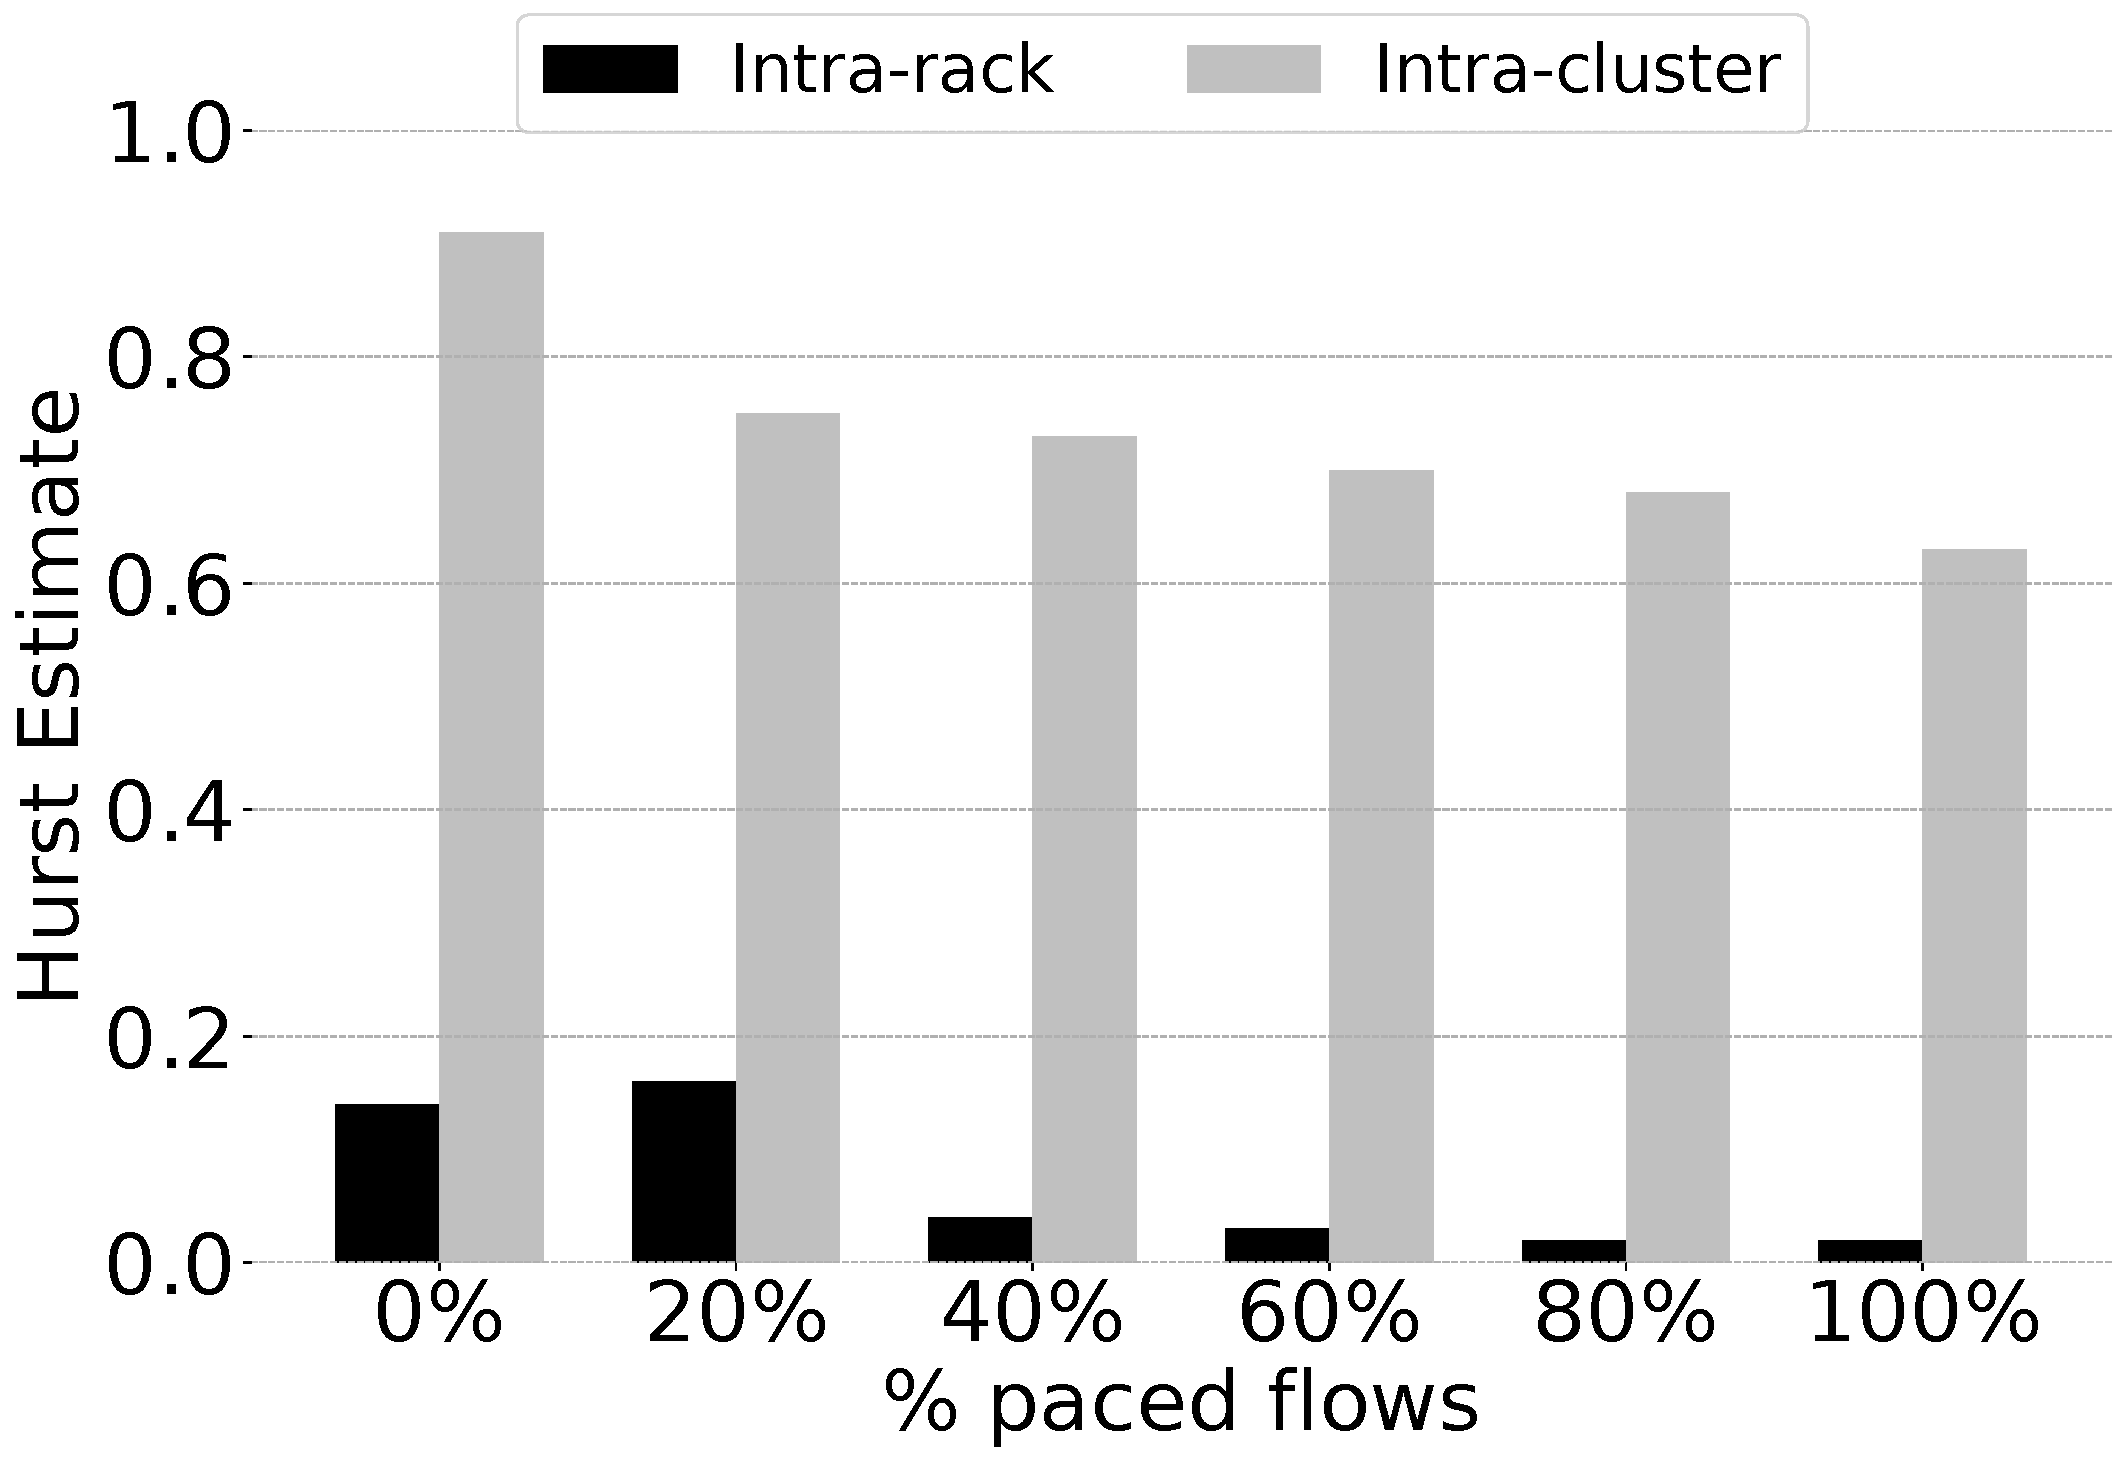
\includegraphics[width=1\linewidth]{figs/pacing_hurst_bar.pdf}
% 			\vspace{-2mm}
%     \end{subfigure}
%  \vspace{-2mm}
%     \caption{\small{\textbf{Comparing the Hurst exponents when we gradually increase the percentage of paced flows for two workloads.}}}
%         \label{fig:app-pacing-hurst}
% \end{figure}

\begin{figure*}[t]
	\centering
	\begin{subfigure}[t]{.24\linewidth}
		\centering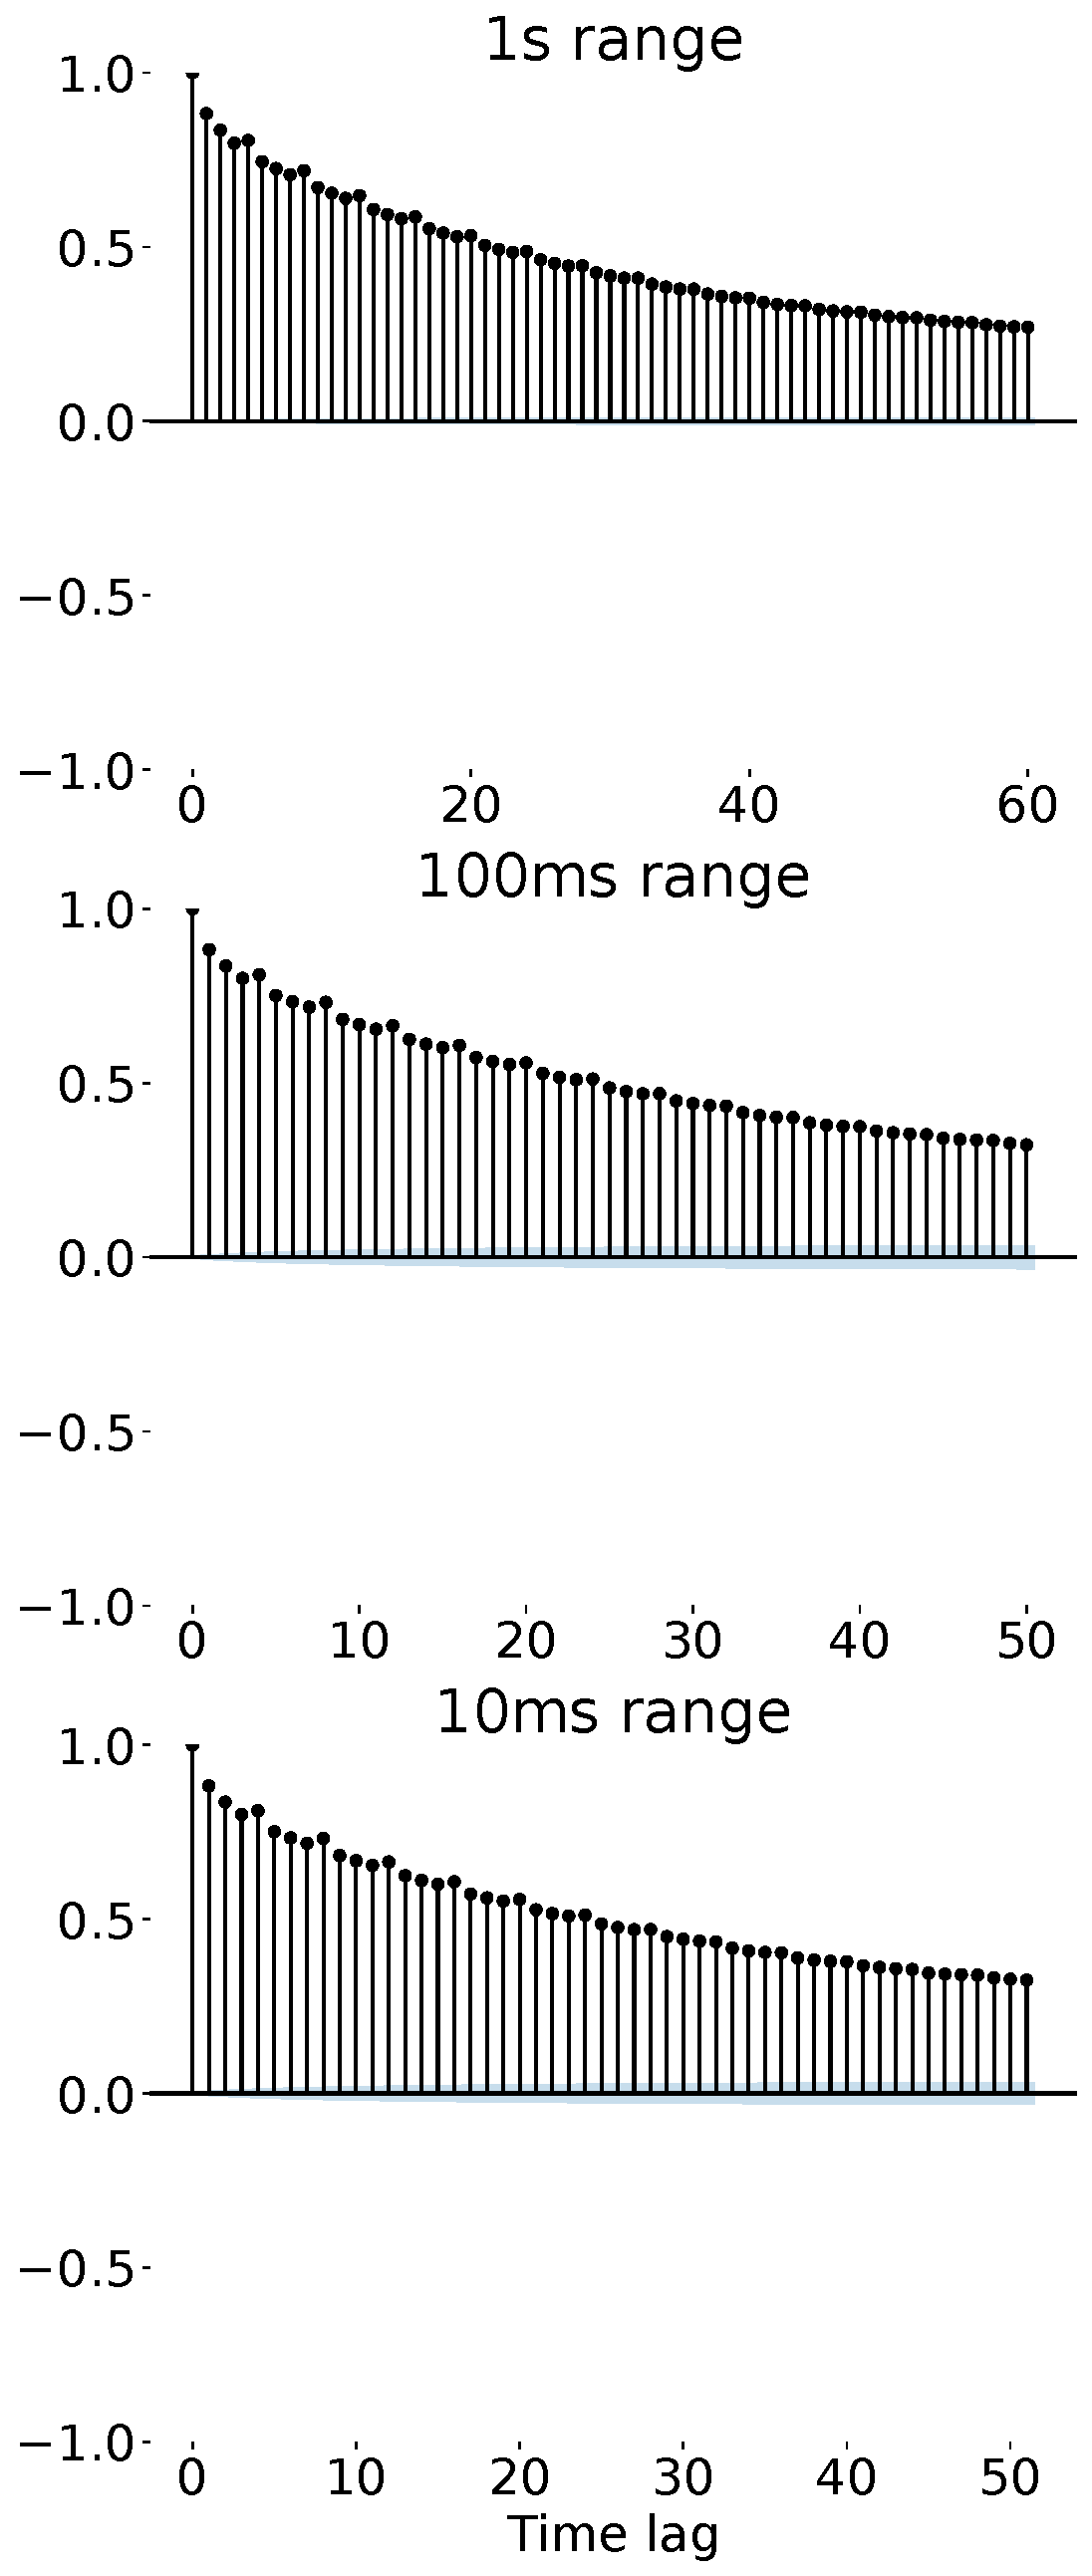
\includegraphics[width=1\linewidth]{figs/intra_cluster_autocor.pdf}
		\vspace{-6mm}
		\caption{\textbf{IC 0\% paced}}
		\label{fig:app-pacing-autocorr-cluster}
	\end{subfigure}
 \begin{subfigure}[t]{.24\linewidth}
		\centering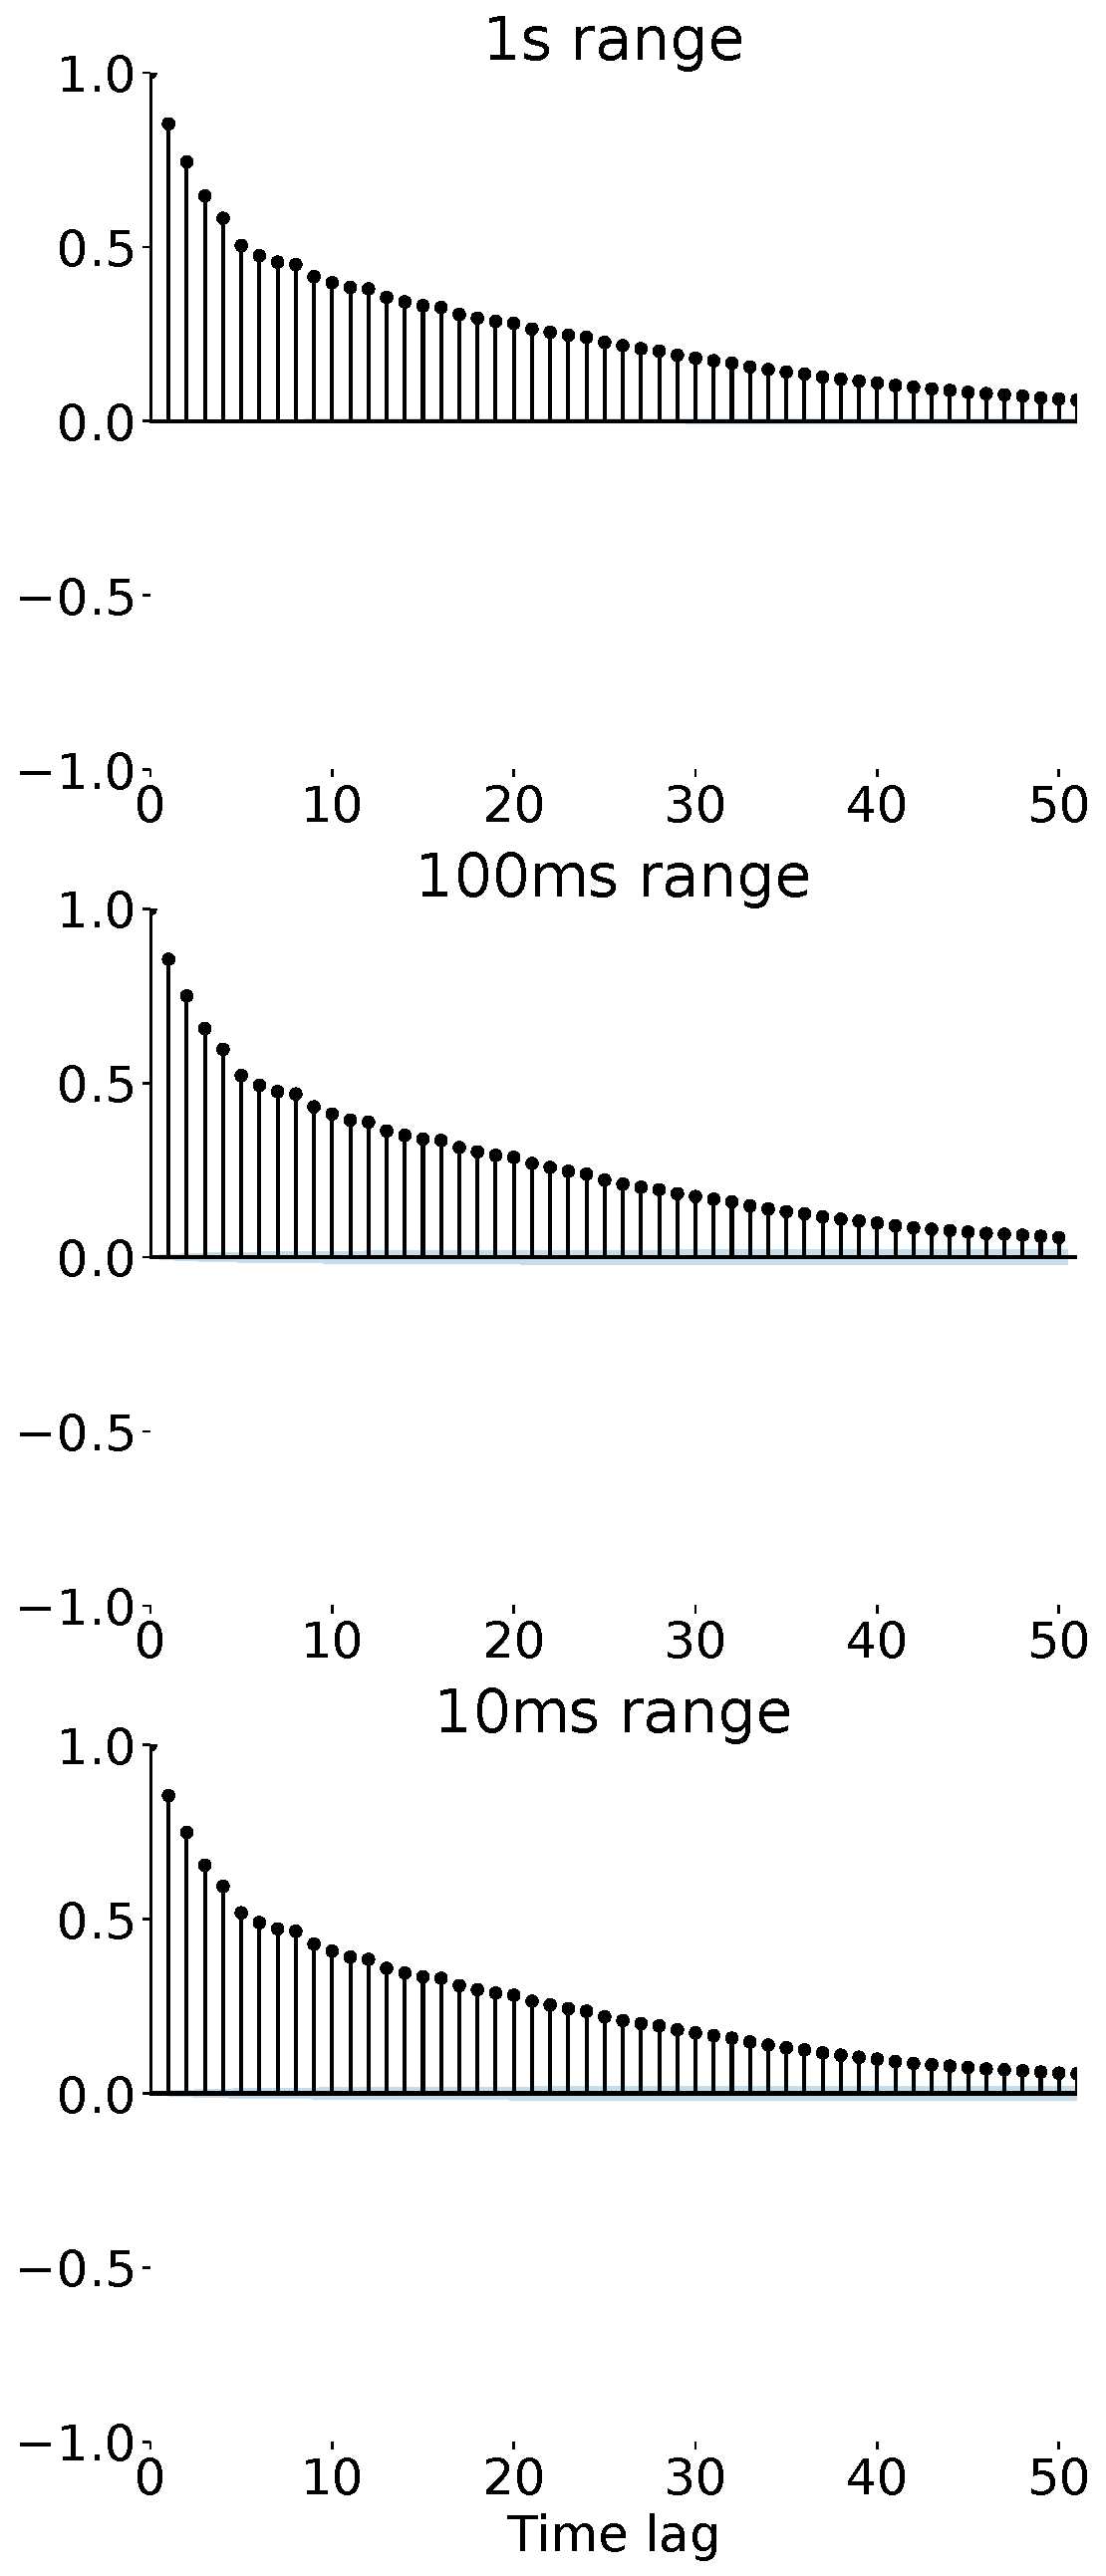
\includegraphics[width=1\linewidth]{figs/intra_cluster_autocor_20.pdf}
		\vspace{-6mm}
		\caption{\textbf{IC 20\% paced}}
		\label{fig:app-pacing-autocorr-cluster-20}
	\end{subfigure}
  \begin{subfigure}[t]{.24\linewidth}
		\centering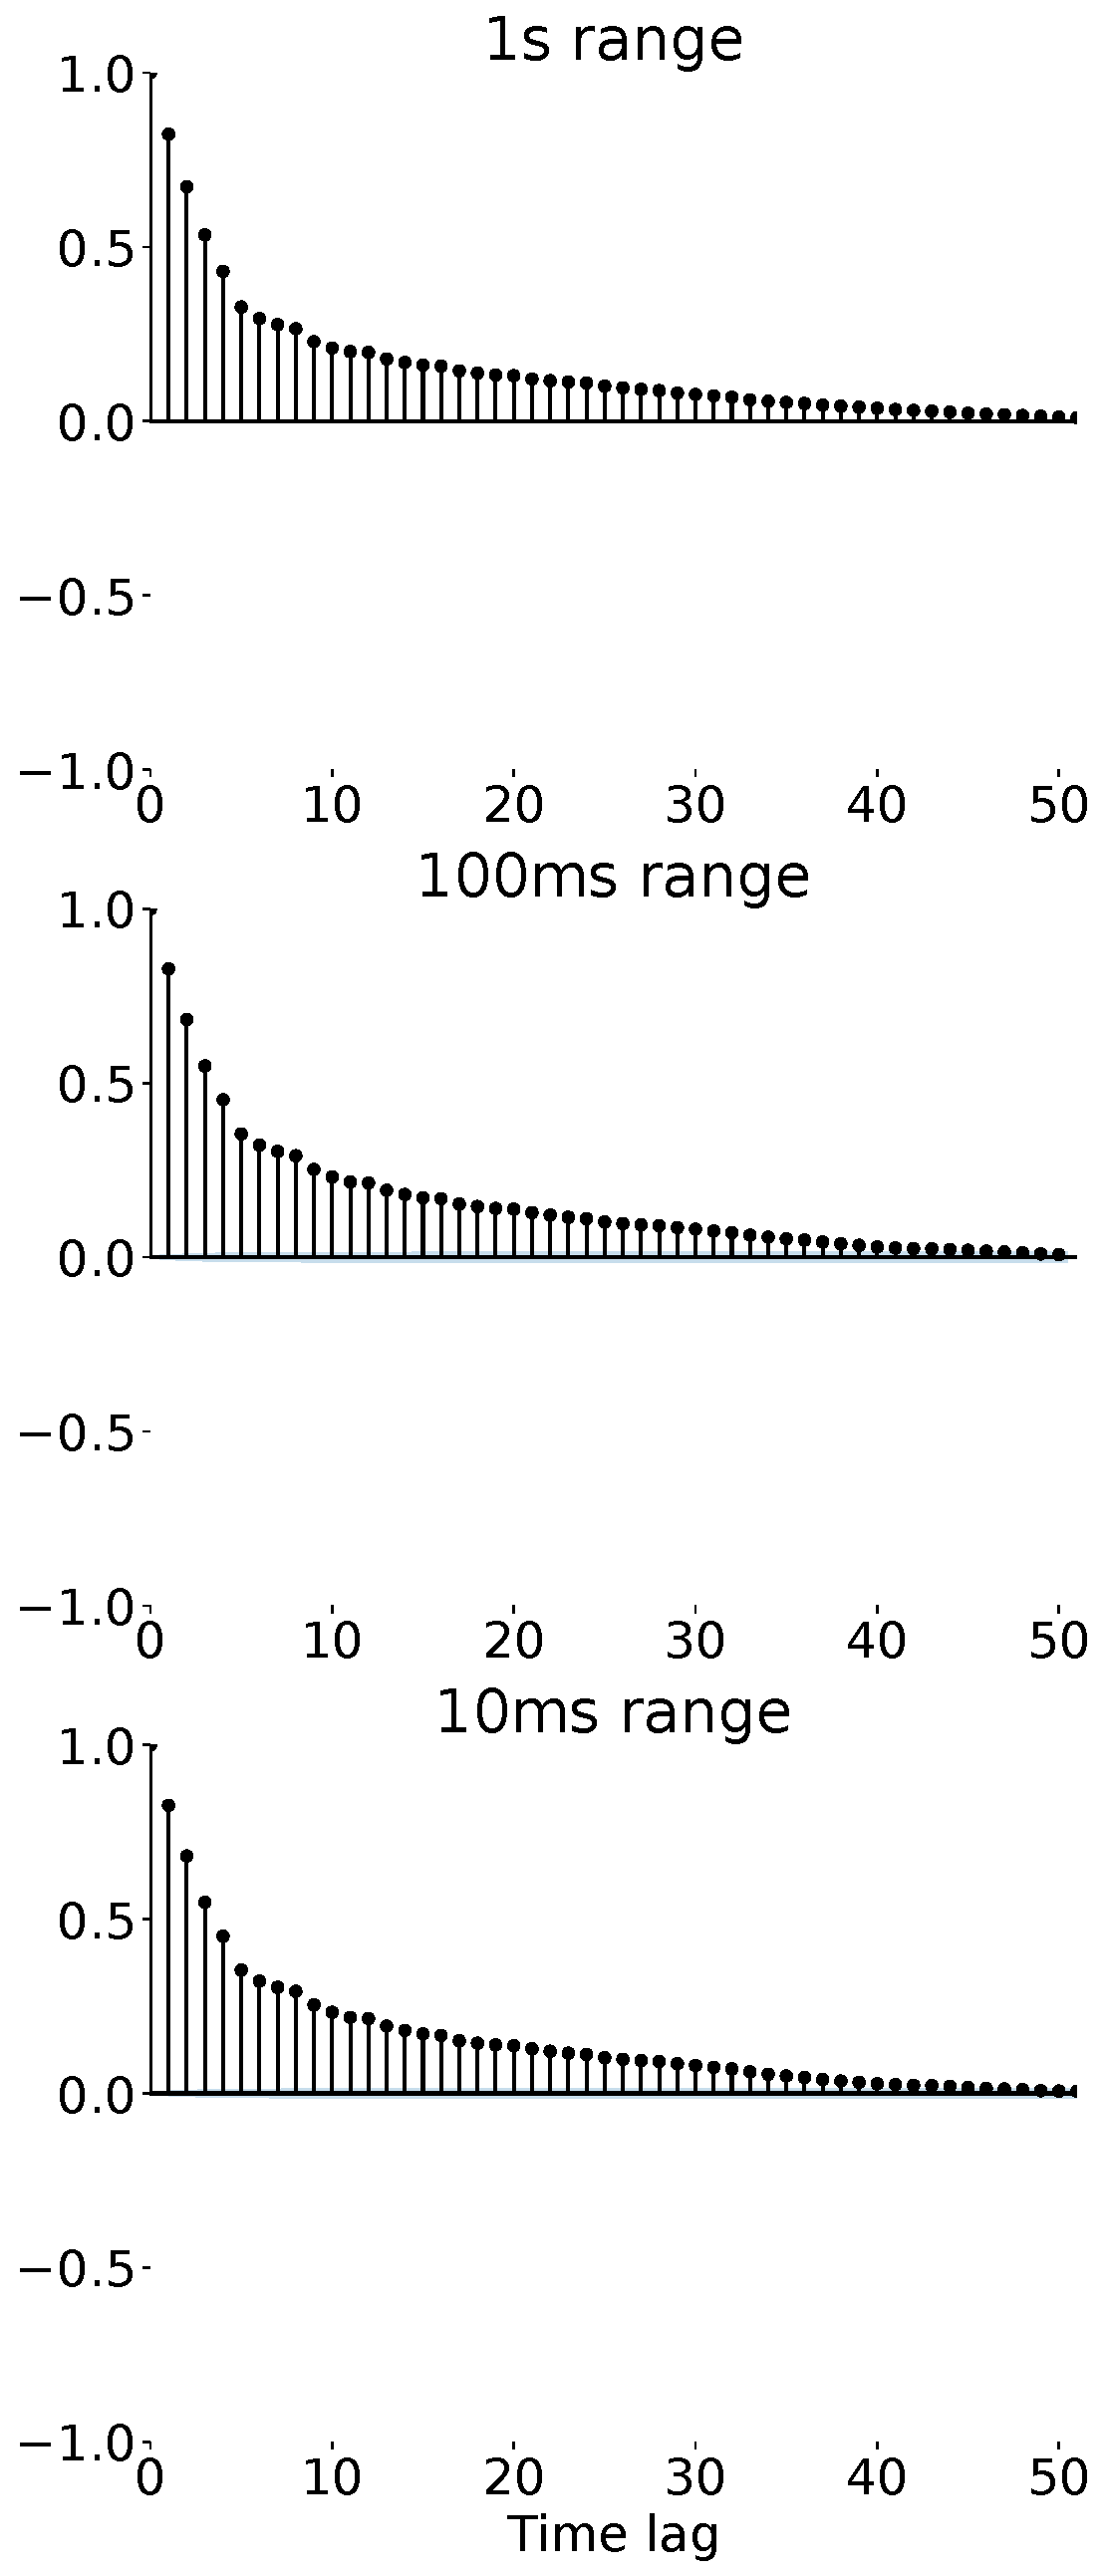
\includegraphics[width=1\linewidth]{figs/intra_cluster_autocor_60.pdf}
		\vspace{-6mm}
		\caption{\textbf{IC 60\% paced}}
		\label{fig:app-pacing-autocorr-cluster-60}
	\end{subfigure}
 	\begin{subfigure}[t]{.24\linewidth}
		\centering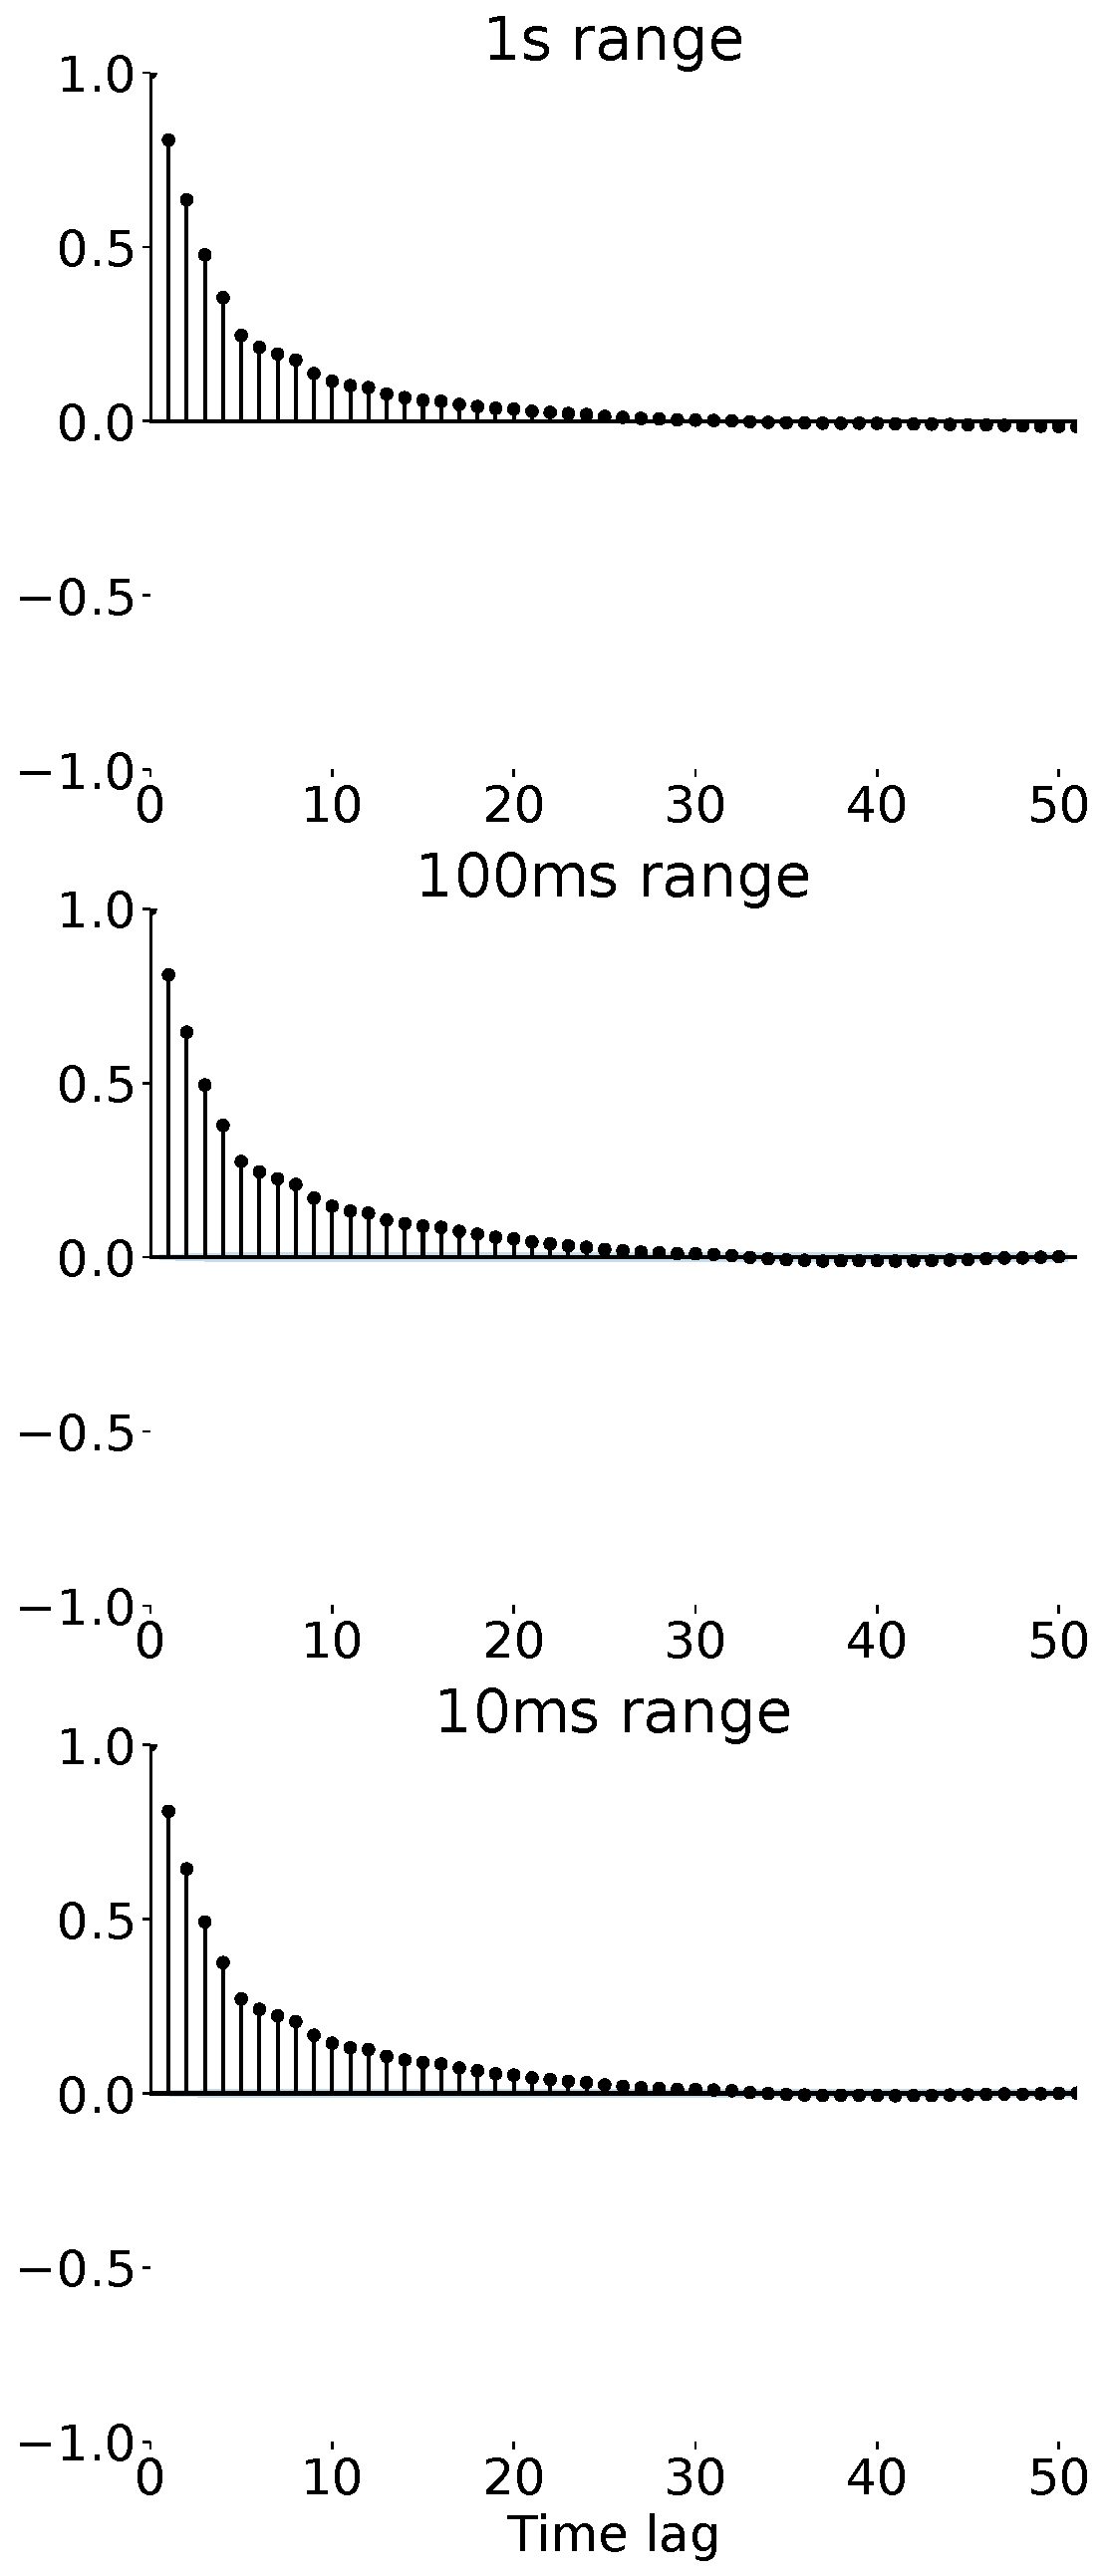
\includegraphics[width=1\linewidth]{figs/intra_cluster_autocor_100.pdf}
		\vspace{-6mm}
		\caption{\textbf{ 100\% paced}}
		\label{fig:app-pacing-autocorr-cluster-100}
	\end{subfigure}
     \begin{subfigure}[t]{.24\linewidth}
		\centering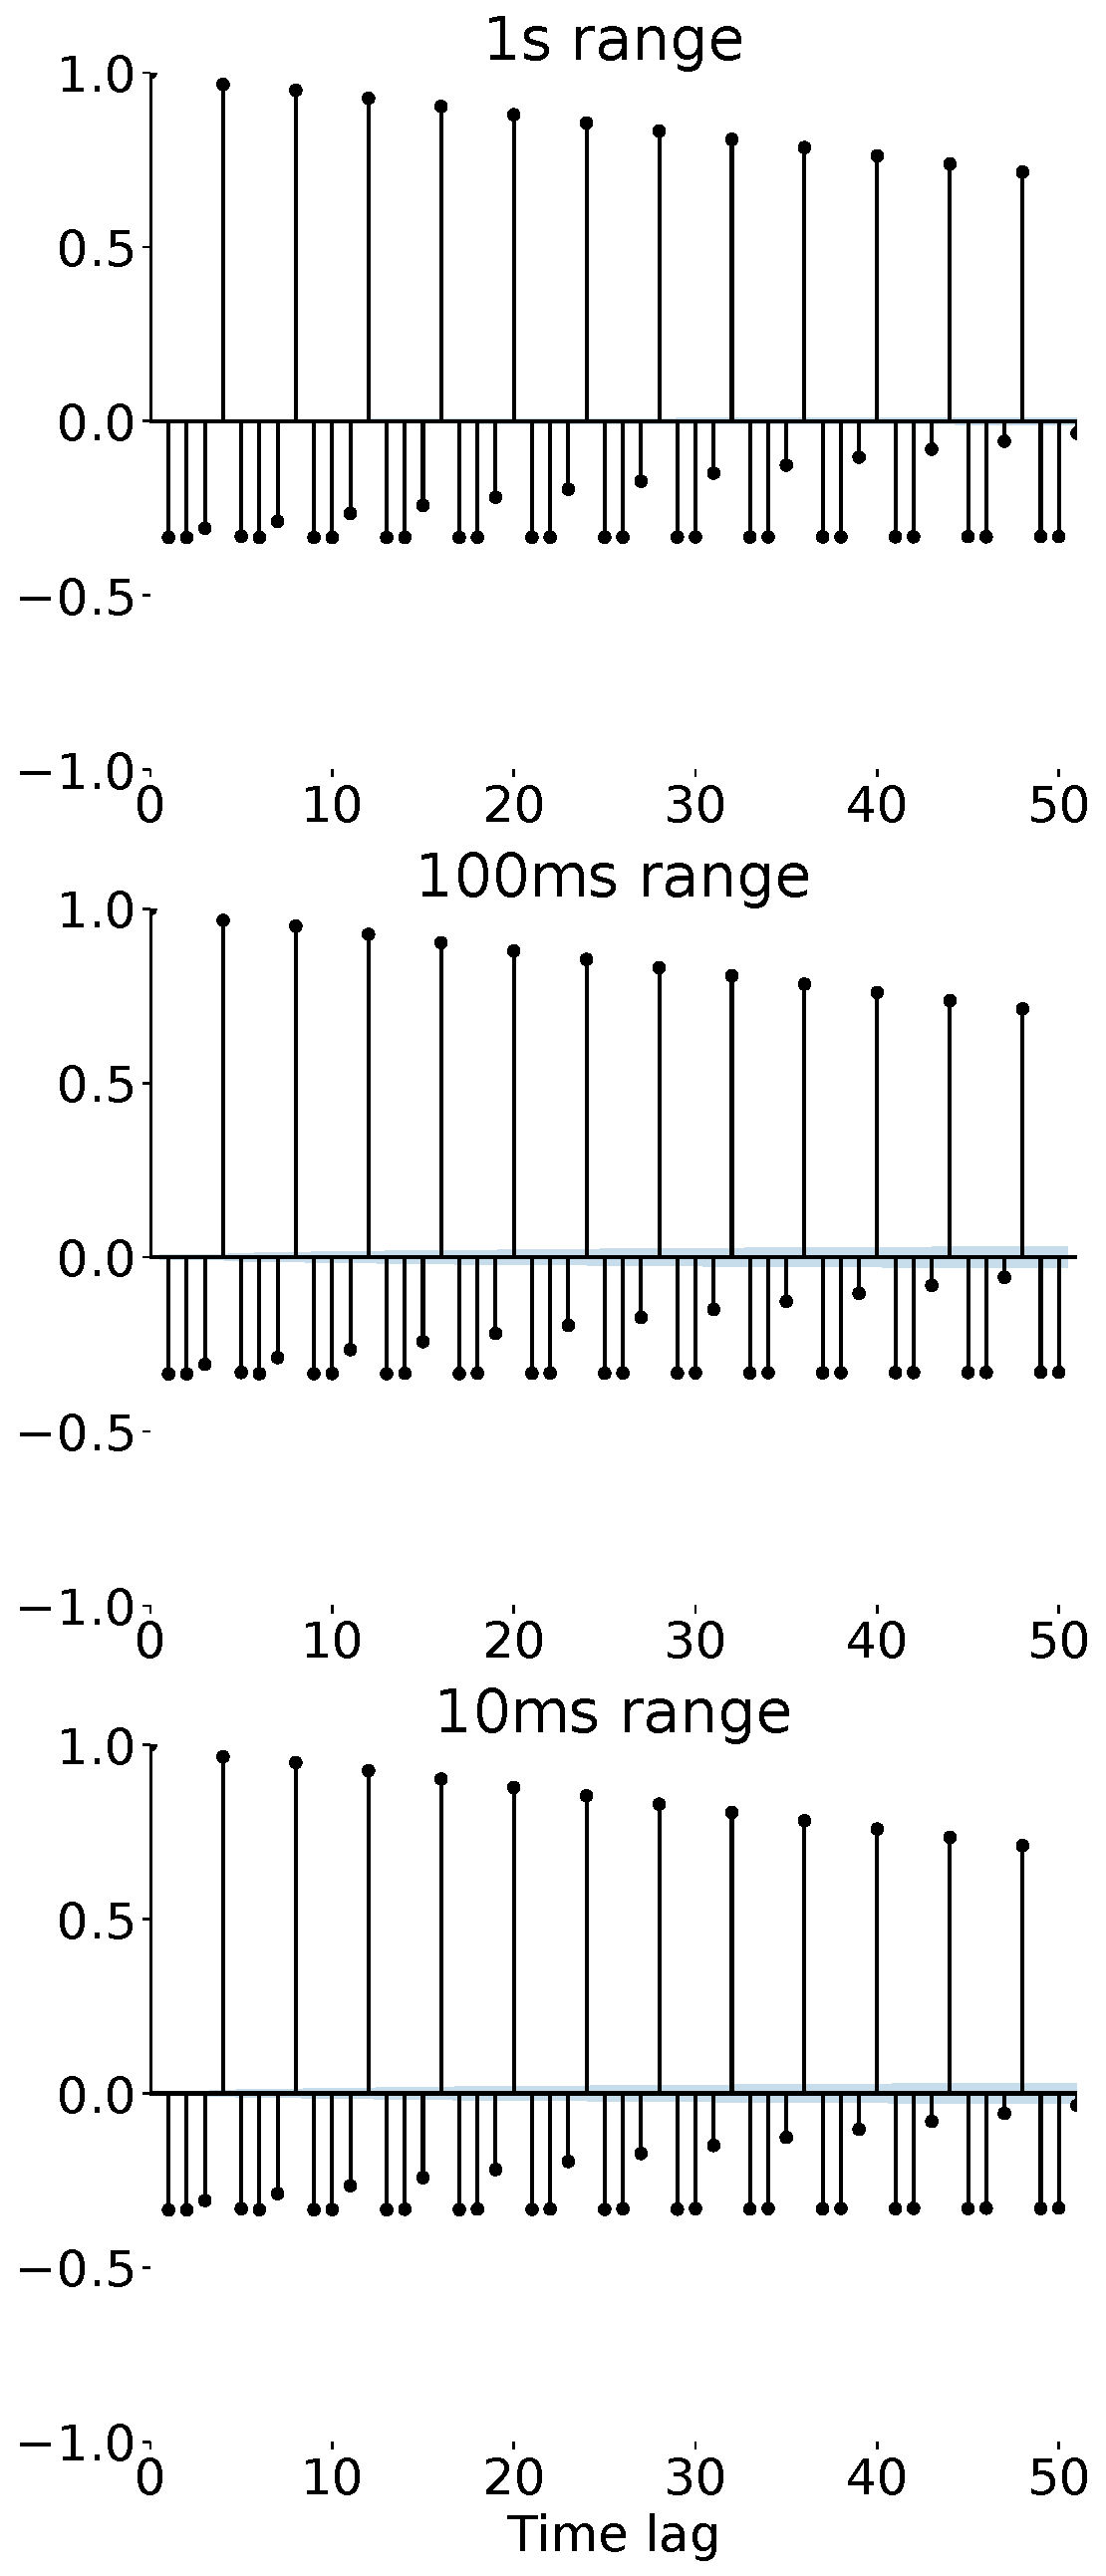
\includegraphics[width=1\linewidth]{figs/intra_rack_autocor.pdf}
		\vspace{-6mm}
		\caption{\textbf{IR 0\% paced}}
		\label{fig:app-pacing-autocorr-rack}
	\end{subfigure}
     \begin{subfigure}[t]{.24\linewidth}
		\centering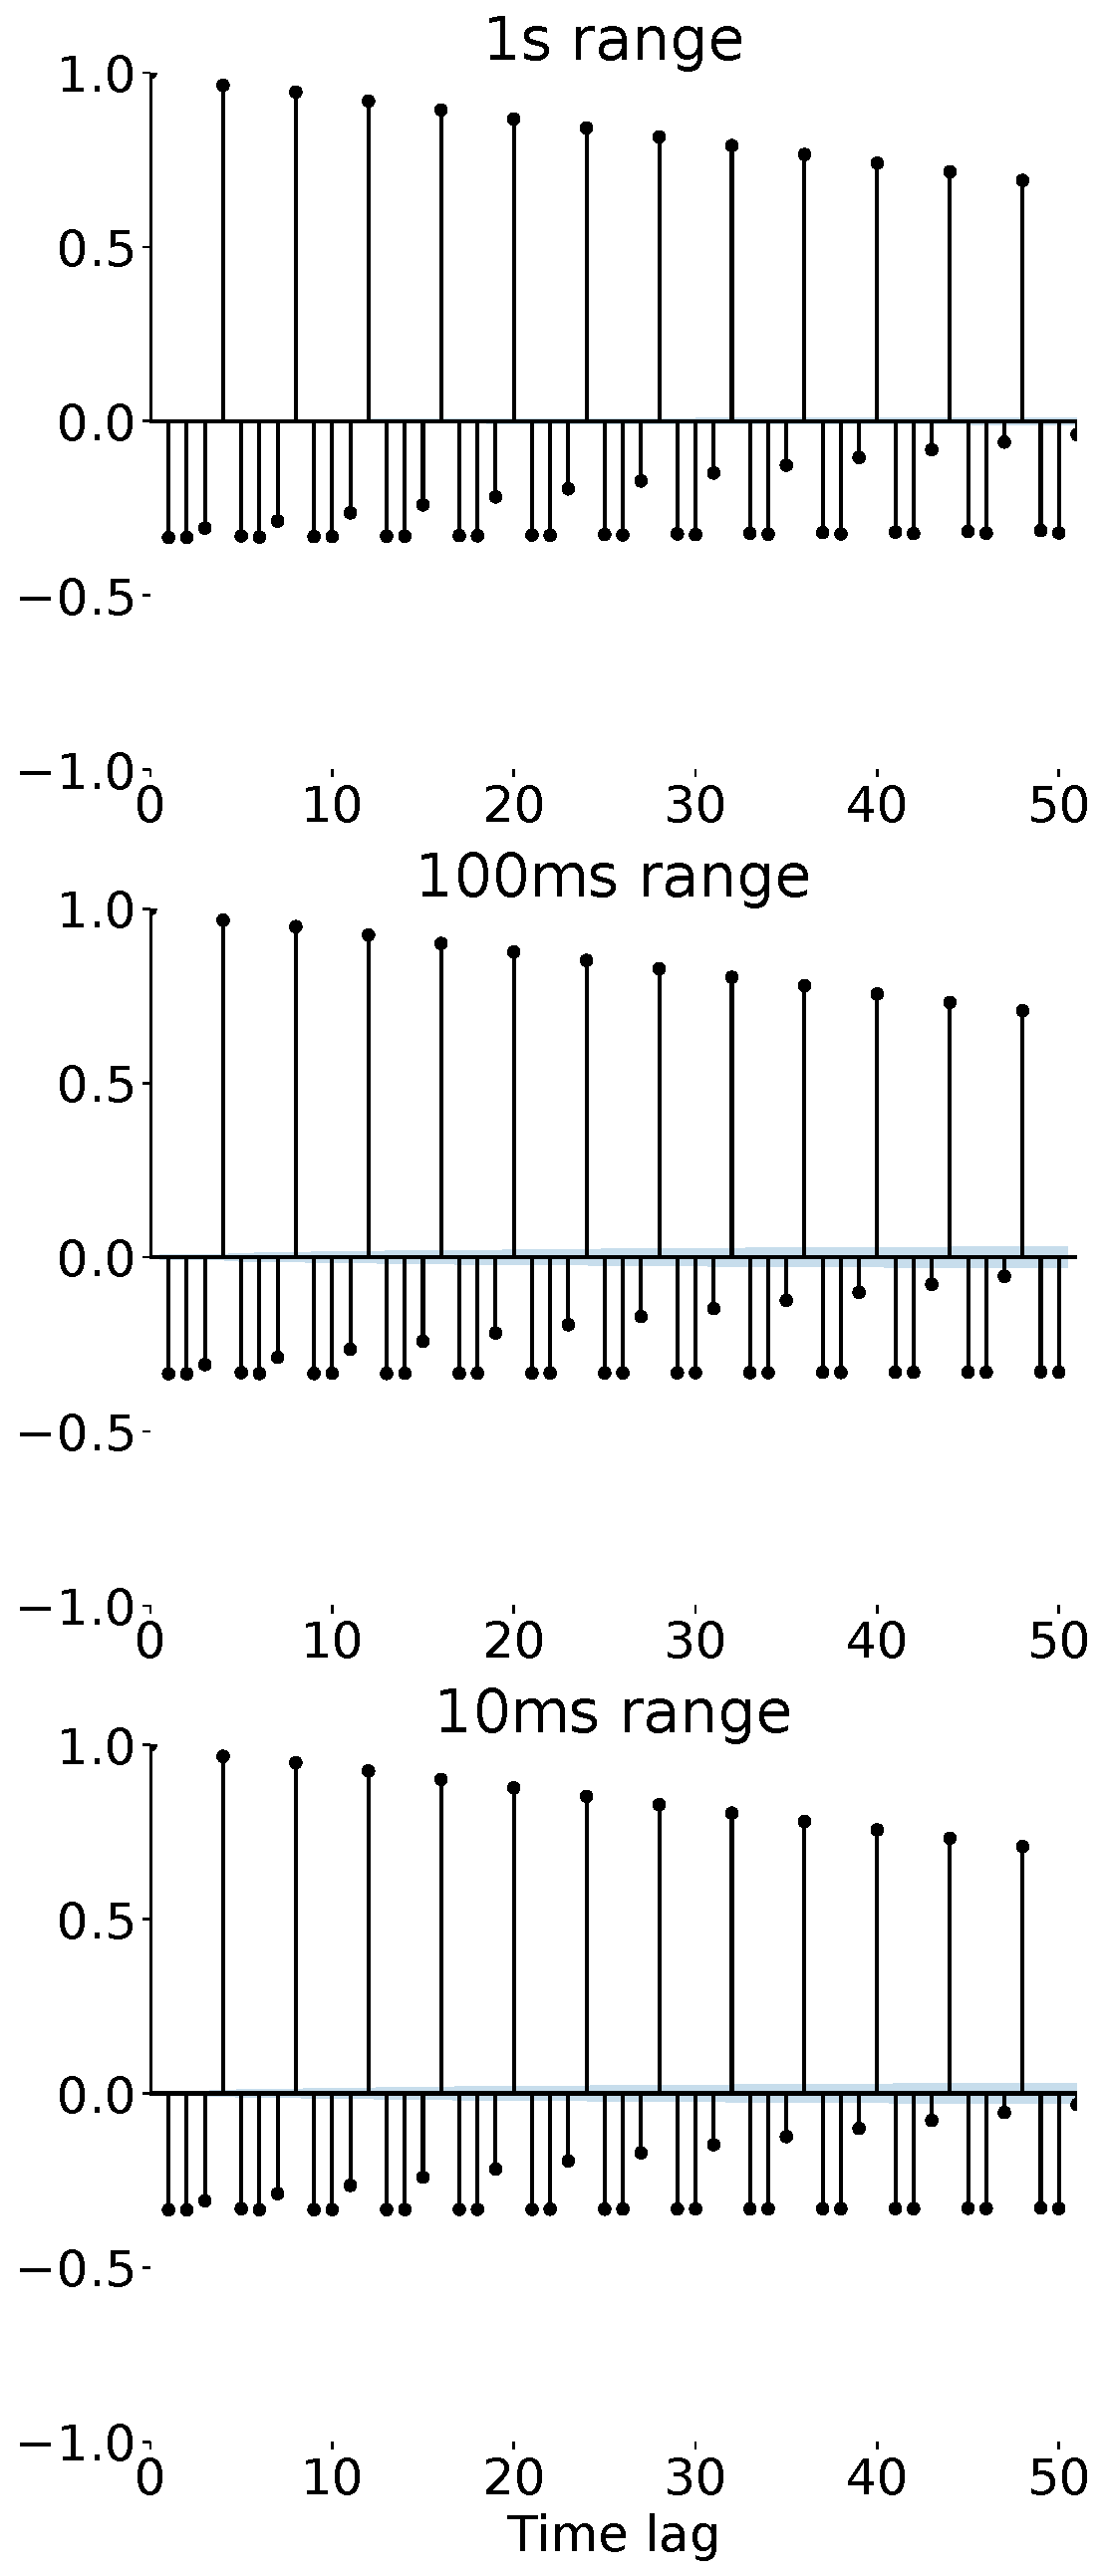
\includegraphics[width=1\linewidth]{figs/intra_rack_autocor_20.pdf}
		\vspace{-6mm}
		\caption{\textbf{IR 20\% paced}}
		\label{fig:app-pacing-autocorr-rack-20}
	\end{subfigure}
     \begin{subfigure}[t]{.24\linewidth}
		\centering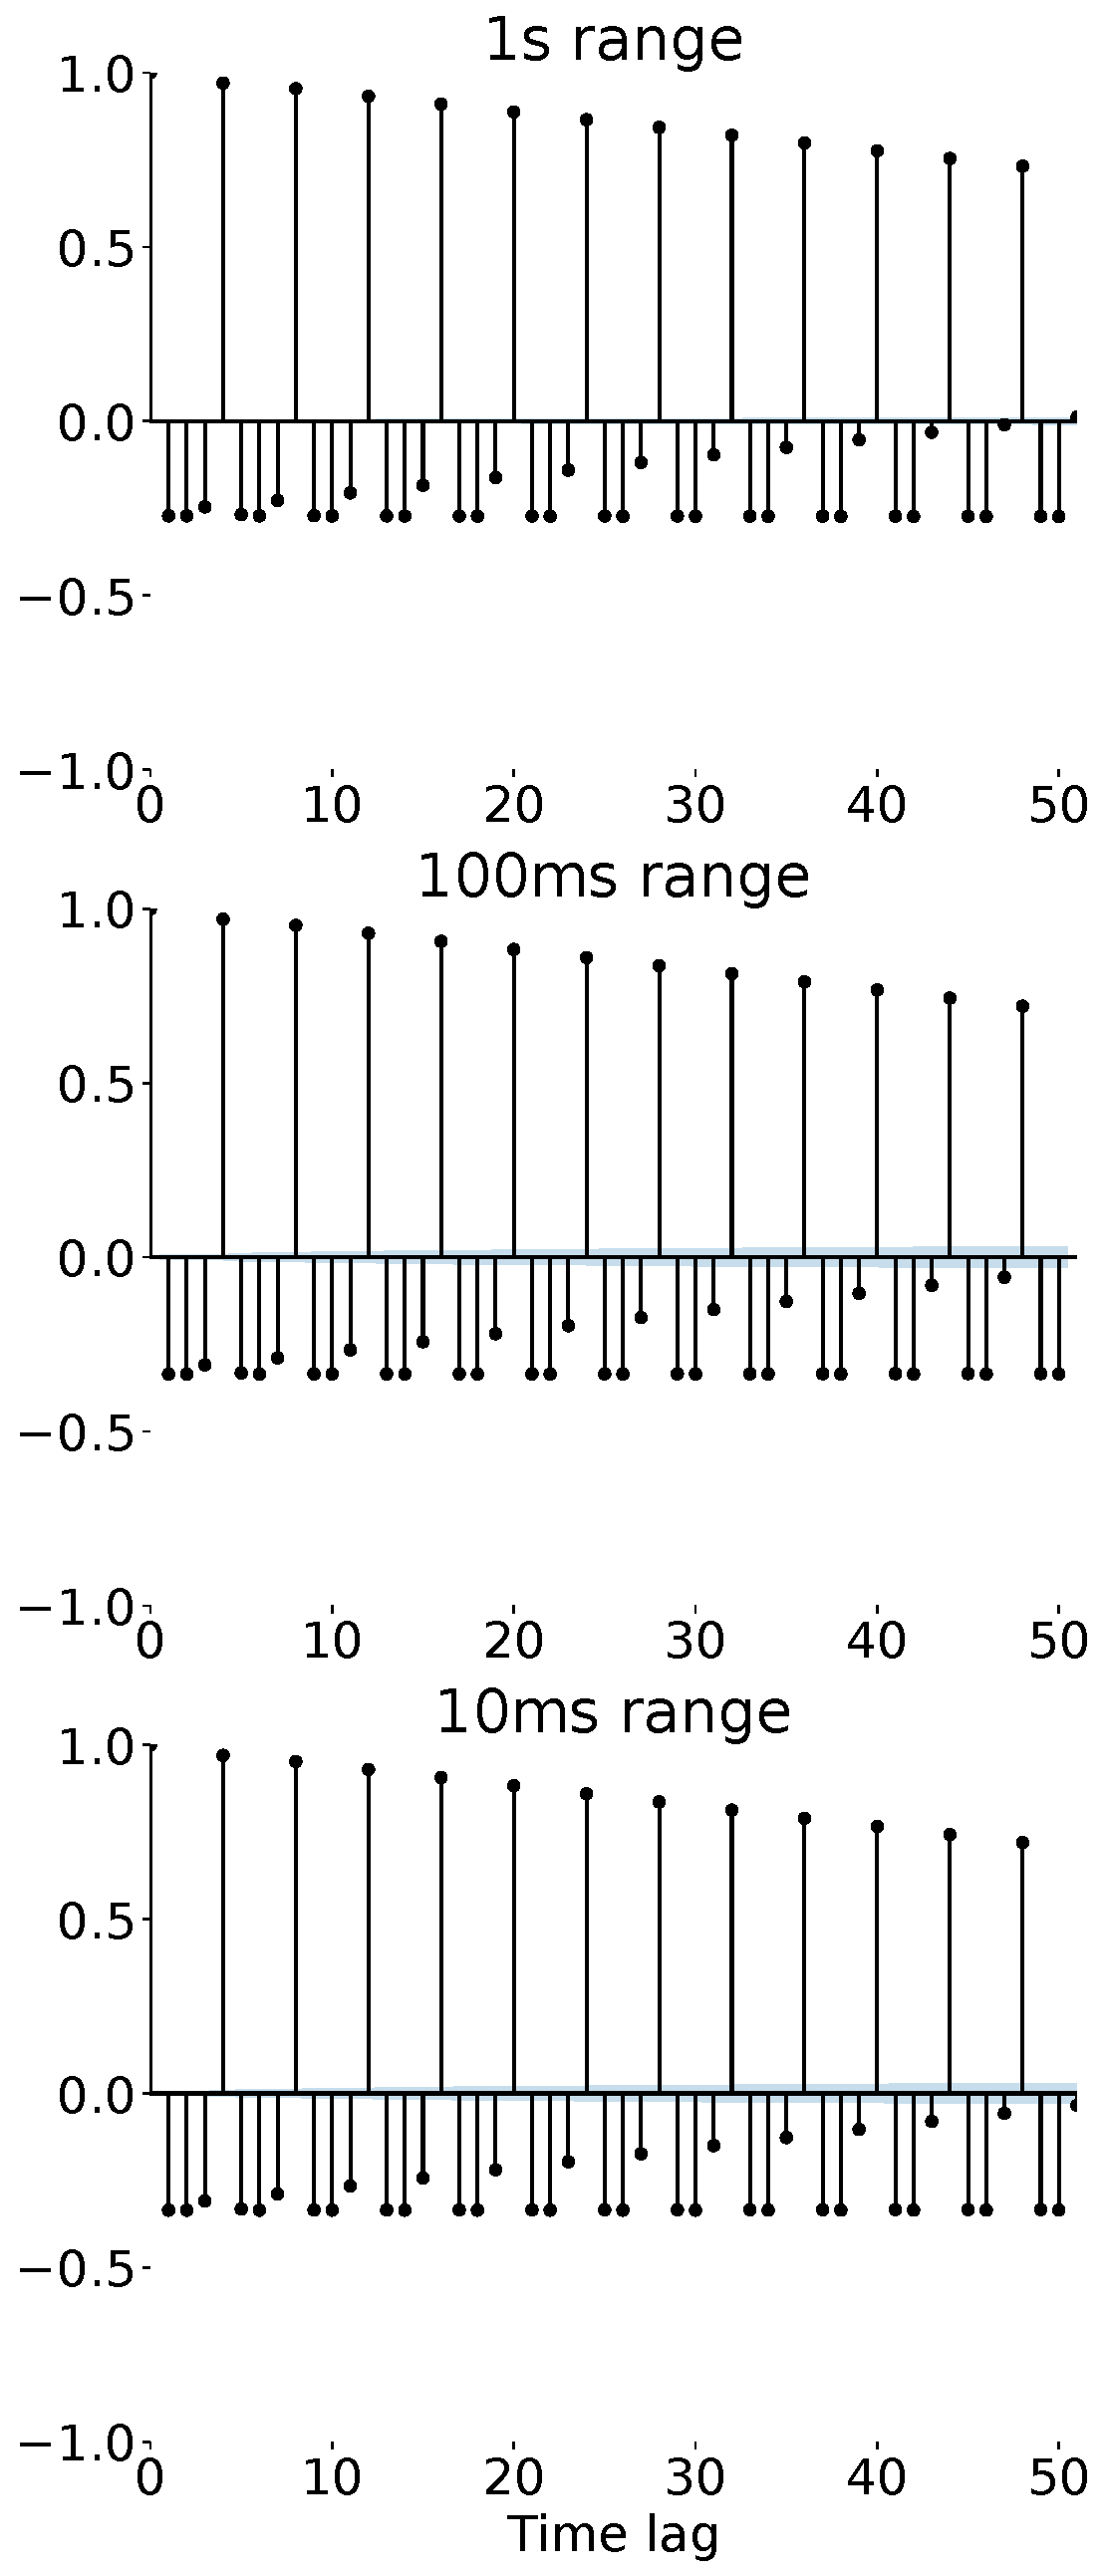
\includegraphics[width=1\linewidth]{figs/intra_rack_autocor_60.pdf}
		\vspace{-6mm}
		\caption{\textbf{IR 60\% paced}}
		\label{fig:app-pacing-autocorr-rack-60}
	\end{subfigure}
     \begin{subfigure}[t]{.24\linewidth}
		\centering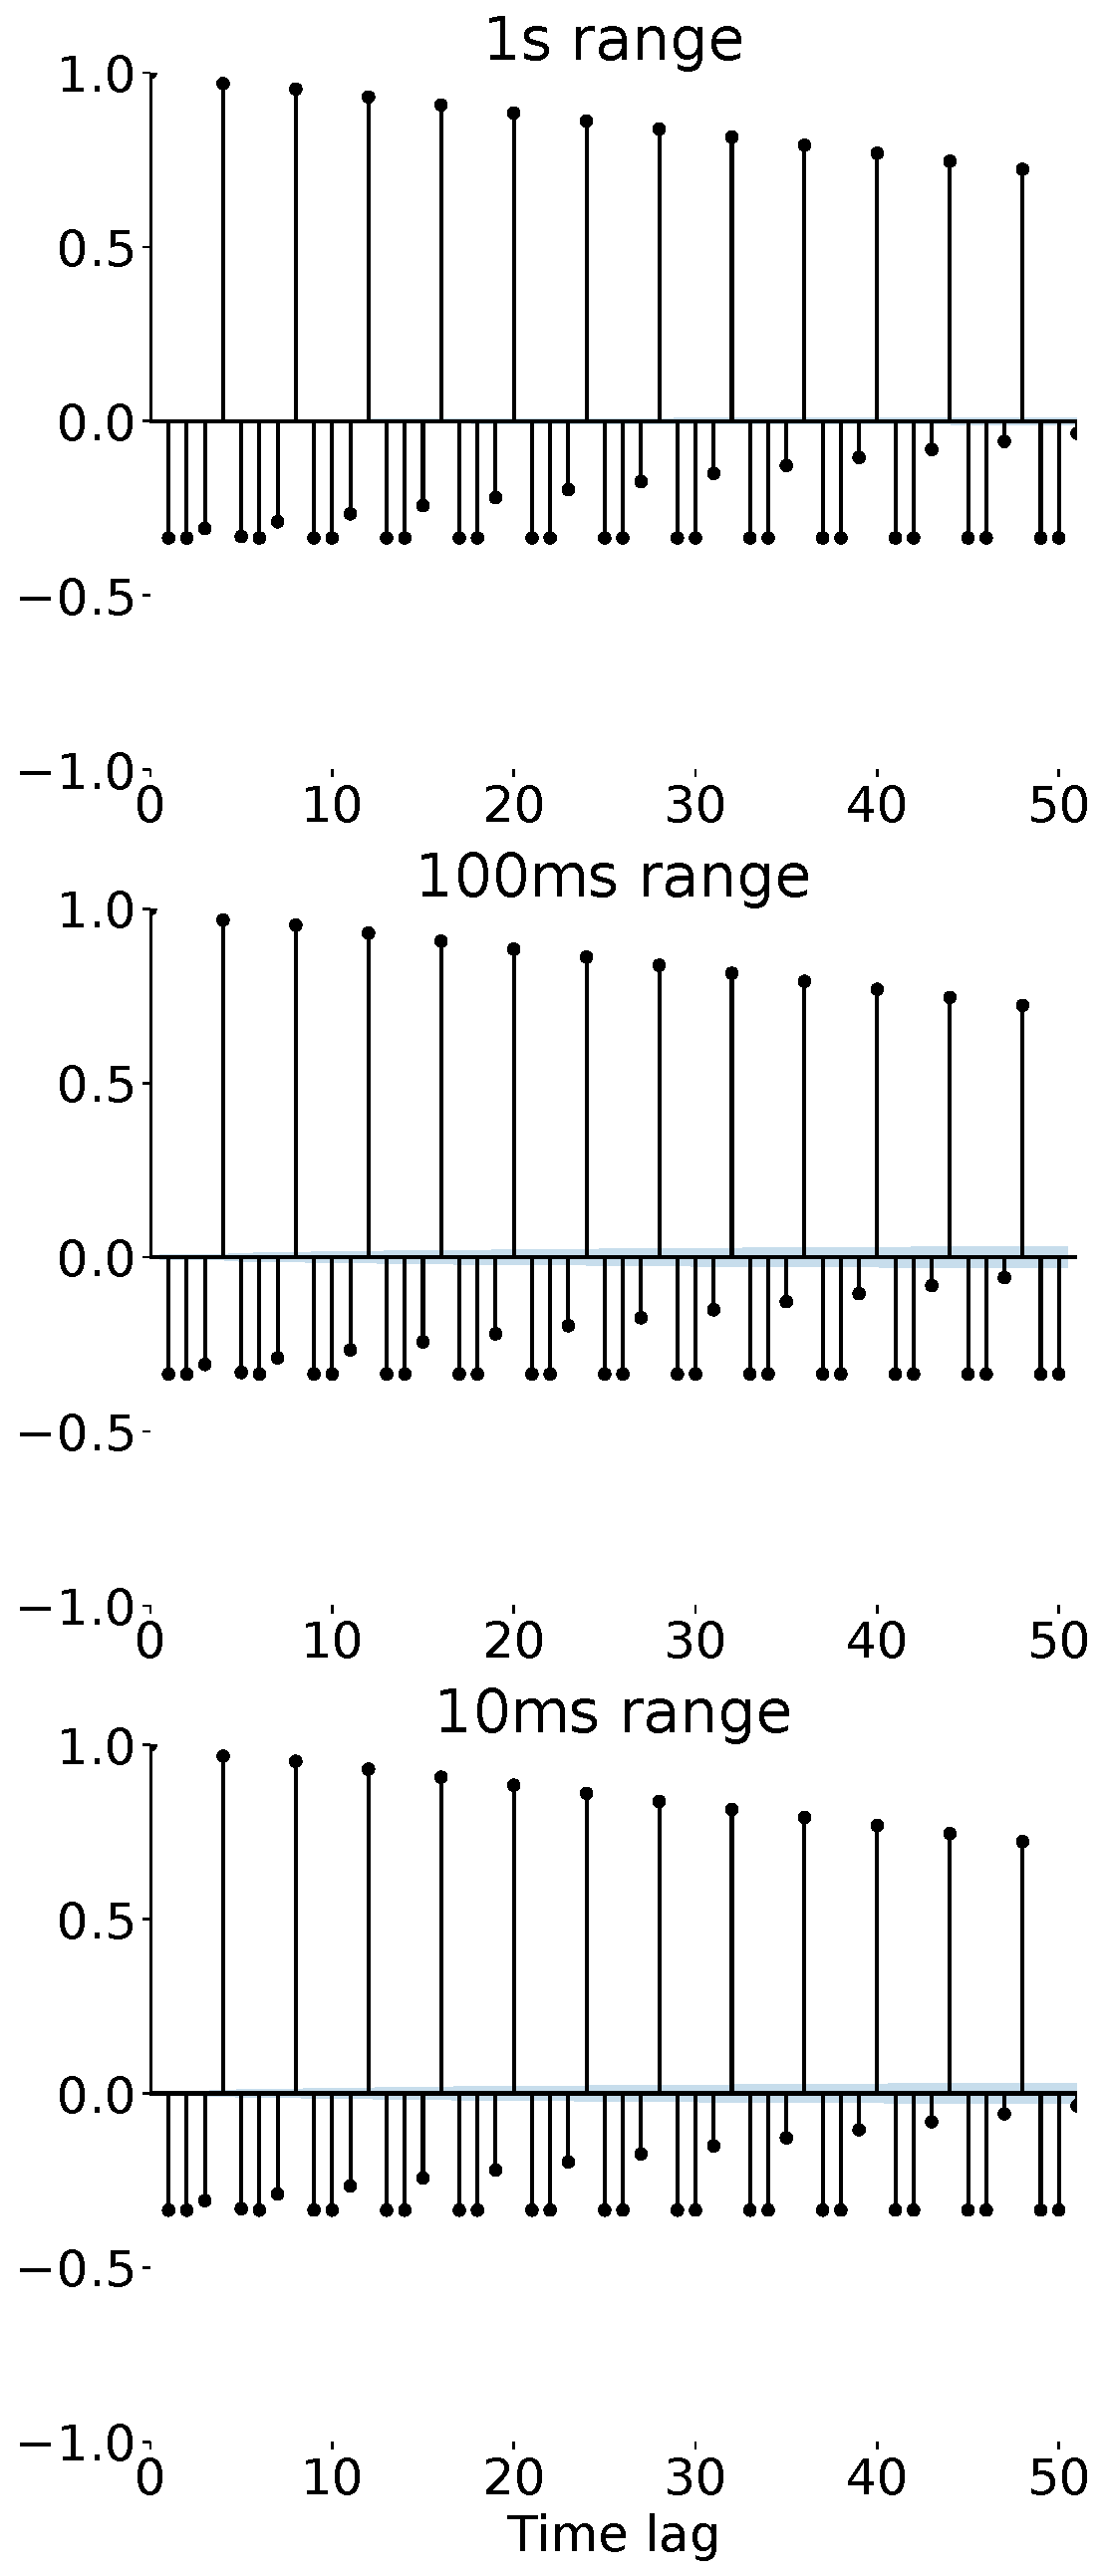
\includegraphics[width=1\linewidth]{figs/intra_rack_autocor_100.pdf}
		\vspace{-6mm}
		\caption{\textbf{IR 100\% paced}}
		\label{fig:app-pacing-autocorr-rack-100}
	\end{subfigure}
\vspace{-2mm}
	\caption{\small{
 Comparing the auto-correlation functions (ACFs) for intra-cluster (IC) and intra-rack (IR) workloads when we increase the ratio of paced flows from 0\% to 100\%. }}
		\label{fig:app-pacing}
	% \vspace{-1em}
\vspace{-2mm}
\end{figure*}
\thispagestyle{empty}


Finally, Figure \ref{fig:app-pacing} presents the corresponding auto-correlation functions (ACFs) for the above time series. While the cycling trend of bars between positive and negative correlations suggests a strong mean-reverting behavior for the intra-rack workload (Figures \ref{fig:app-pacing-autocorr-rack}-\ref{fig:app-pacing-autocorr-rack-100}), the intra-cluster ACF features a slow-decaying, strong positive correlations across time lags, suggesting strong self-similarity (Figures \ref{fig:app-pacing-autocorr-cluster}-\ref{fig:app-pacing-autocorr-cluster-100}). As we increase the pacing ratio (from 0\% gradually to 100\%), the correlations start to decline.

\thispagestyle{empty}
